\documentclass[titlepage,11pt]{article}
\usepackage{fullpage}
\usepackage{graphicx}
\usepackage{titlesec}
\usepackage{float}
\usepackage{subfig}
\usepackage[demo]{rotating}
\usepackage{listings}
\usepackage{hyperref}
\usepackage{cite}

\newcommand{\sectionbreak}{\clearpage}
\setcounter{secnumdepth}{4}
\setcounter{tocdepth}{4}
\setlength\parindent{0pt}

\titleformat{\paragraph}{\normalfont\normalsize\bfseries}{\theparagraph}{1em}{}
\titlespacing*{\paragraph}{0pt}{3.25ex plus 1ex minus .2ex}{1.5ex plus .2ex}

\begin{document}
\pagenumbering{gobble}
\title{VISiBLE - Visual Steerable Symbolic Execution}
\author{Feroz Jilla, Radu Szasz, Amey Kusurkar \\ Eugenia Kim, Jason Yu, Vaibhav Krishnakumar \\ Supervised by: Antonio Filieri \\ Special thanks to Mateus Araujo Borges}
\date{}

\begin{figure}
\centering

\includegraphics[scale=0.5]{crest.png}
\end{figure}

\maketitle 
\newpage
\section*{Executive Summary}

As programmers, we have all used unit testing. Yet, we all know that even a great set of unit tests does not guarantee a bug free program.
It is just too hard to generate tests that cover all the possible execution paths your program could follow. Coverage testing can identify the
untested parts, but even then there is a lot left to be desired. How would you generate a test case that follows exactly the path you want to test? \\

It is a hard thing to do, unless you have symbolic execution on your side. Java Path Finder is one such tool which not only tests code on
a set of pre-defined inputs, but on all of them. (If you think that would mean a lot of states and a lot of overhead, you are right.) \\

This is why VISiBLE brings the power of symbolic execution to you via a simple user interface. Every possible path in any program, with any number
of \texttt{if}s, \texttt{while}s or \texttt{for} loops can be explored in just a few clicks. All VISiBLE requires is a \texttt{jar} file and the magic begins! \\

The user can focus on the decision points in the code. Unlike execution with concrete variables, there is no predetermined path the execution will follow.
It's up to the user to take the wheel and steer the program left and right. \\

What’s the benefit of this? \\

At every point of this quick easy process, we display a path condition - the restrictions that apply on your variables in order to follow the path our user did while navigating the tree. And we do not stop here: we provide a variable assignment that would cause a test to follow exactly the same path
as our user did. \\

No more struggles in achieving 100\% test coverage; no more bugs. Well, almost... you know what they say: there is always one more bug! Find it. Fix it. \\

VISiBLE!

\tableofcontents

\section{Introduction}
\pagenumbering{arabic}
\setcounter{page}{1}
VISiBLE stands for Visual Steerable Symbolic Execution. Given a Java program, VISiBLE allows the user to visualise and steer the symbolic execution of the program. The execution is represented in the form of a tree, with every node representing a binary decision point in the program (such as an \texttt{if/else} statement).

\subsection{What is Symbolic Execution?}

Symbolic Execution is an analytic way of running a program that replaces input parameters with symbolic values, producing an output in terms of these values. This is in contrast to running a program normally with actual inputs, where the program follows a fixed linear execution path based on the values of the inputs. When a program is executed symbolically, it essentially takes \textit{every possible} execution path, branching at decision points in the program. This results in an execution path tree, as seen in Figure \ref{fig:symex}. \\

\begin{figure}[H]
\centering
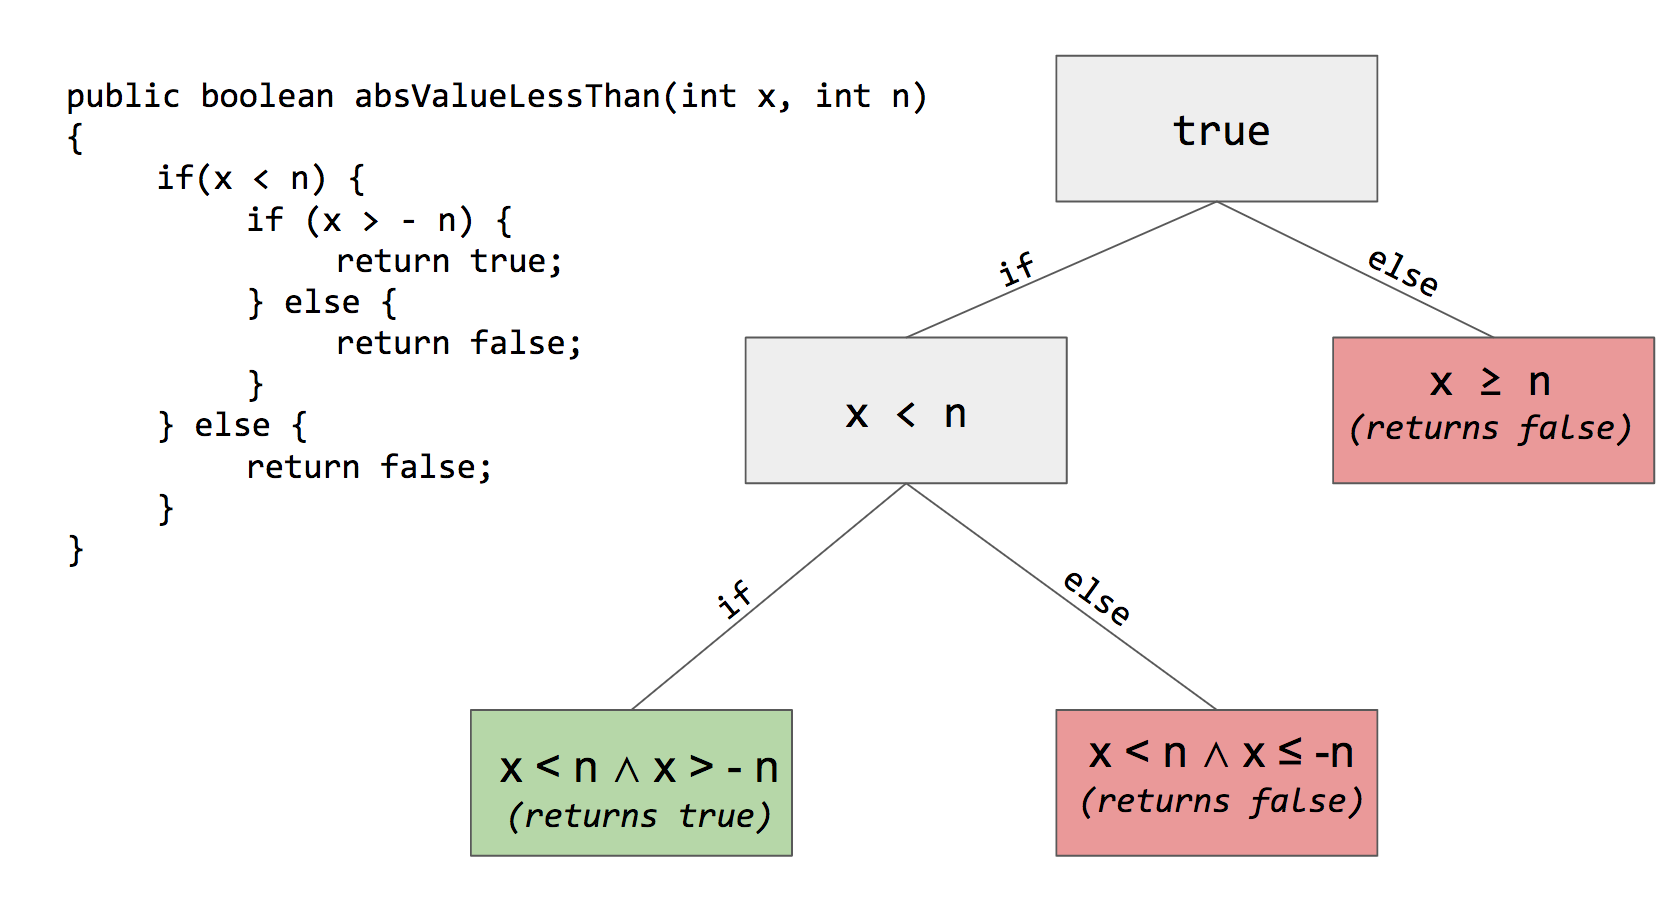
\includegraphics[scale=0.5]{symex.png}
\caption{Execution path tree of the symbolic execution of a function}
\label{fig:symex}
\end{figure}

Figure \ref{fig:symex} shows the execution path tree for \texttt{absValueLessThan} with symbolic values for \texttt{x} and \texttt{n}. The nodes in the tree represent the decision points in program, with the branches corresponding to picking the \texttt{if} and \texttt{else} cases. The logical statement shown in each node corresponds to the conditions that must hold for execution to have reached that node. This is called the \textit{path condition}. In other words, the path conditions tell us the range of values that the symbolic inputs can take at each point in the execution. Notice that if we had used concrete inputs instead, the values of the inputs would be known at each point in the program, making the execution path deterministic. Hence there would be no branching, as there is no decision to be made. \\

Looking at the symbolic execution tree, it becomes clear which values of \texttt{x} and \texttt{n} would return true and which would return false. As for the example in Figure \ref{fig:symex}, if we look at the path condition required to return true, it becomes obvious that the function is checking if $|x| < n$. Thus, symbolic execution can be used extensively in verification and model-checking.

\subsection{Motivation}
VISiBLE is an interactive web application that is well suited for analysing small to medium sized projects. This would make it useful for programmers who enjoy the activity and pursue it as an interest, mostly for personal projects. Because of the highly computationally intensive task of exploring all possible execution paths, it becomes impractical as a tool for large industrial-grade projects. \\

Within our target group, VISiBLE is beneficial to programmers of all levels, from beginners learning Java through to experienced campaigners eager to start on a new project. We see two key areas of motivation where VISiBLE aims to provide value.

\subsubsection{Testing and Debugging}
For more experienced programmers working on personal projects, testing and debugging are time consuming and tedious parts of the process. VISiBLE aims to reduce the time spent on these activities. The visualisation and steerability features help the programmer understand the code and the control flow of the program, picking up higher level flow errors. \\

Given the difficulty of testing program output on a range of inputs, it is often neglected. Unit-testing can only test a fixed set of inputs with no guarantees to cover all cases. By definition, symbolic execution guarantees full branch coverage as it explores all possible execution paths. We can even determing the concrete inputs that satisfy the exact path conditions of the nodes in the tree, automating test-case generation.

\subsubsection{Educational}
For first time programmers, having a visual representation of the code they write is incredibly useful. By allowing the execution path to be steered, it helps them understand the basics of control flow in a Java program by considering the output symbolic trees for \texttt{if, for} and \texttt{while} statements. Moreover, it aids the understanding of conditions for loop entry and exit, an essential part of the second year 'Reasoning about Programs' course at Imperial College. This is a source of infinite frustration that can potentially be reduced through the use of our visual interface. It also makes it easier to spot the dreaded 'off-by-one' error!

\subsection{Overview}
To aid the exploration of the possible execution paths, VISiBLE uses a tool called Java Path Finder (JPF) \cite{petermehlitz}, and more particularly an extension called Symbolic Path Finder (SPF) \cite{corinapasareanu2016}, which uses JPF to execute programs symbolically. JPF is an open-source project developed by the National Aeronautics and Space Administration (NASA) Ames Research Center.
It makes the computational power of JPF accessible through a web interface while extending its functionality in three key areas to provide a comprehensive tool for steerable symbolic execution. 

\subsubsection{Visualisation}
Visualisation allows programmers to understand the code base in a much neater graphical form - it is much more readable and pleasing on the eye than the coarse text output produced by bare bones JPF.  It allows for better understanding of the control flow in an application; starting from \texttt{main}, the logical structure of the program is made apparent by following a path along the generated tree. VISiBLE allows the user to understand the program inside and out, making modifying and extending the program much easier. 

\begin{figure}
\centering
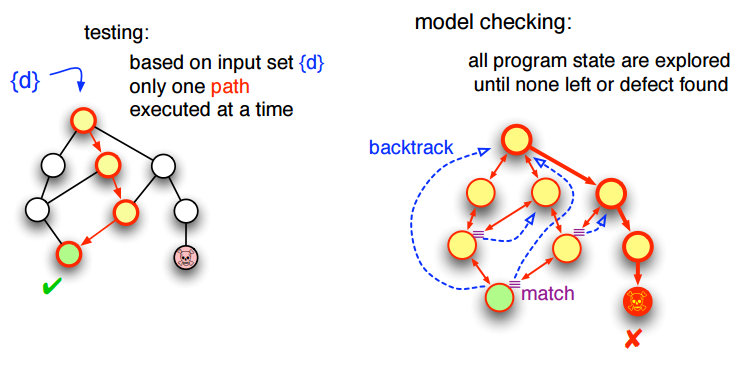
\includegraphics[scale=0.4]{model_checking.png}
\caption{Testing v/s Model Checking \cite{petermehlitz2010}} 
\label{fig:model_checking}
\end{figure}

\subsubsection{Symbolic Execution}
Symbolic execution is a powerful tool that gives programmers greater flexibility than more conventional unit testing. The biggest advantage of symbolic execution is model checking - we can simultaneously check \textit{all} execution paths through a program. This is different from testing, which needs to run multiple test cases for different inputs, and checks one execution path at a time. The diagram in Figure \ref{fig:model_checking} shows this distinction. VISiBLE gives the programmer the output from a comprehensive model checking software which further aids understanding and debugging. This is used to auto-generate test cases that satisfy the constraints generated by VISiBLE, leading to 100\% code coverage. 

\subsubsection{Steerability}
Steerability gives the programmer control over the program at runtime - an invaluable tool to ensure that the behaviour of the program is as expected. At every possible decision point, VISiBLE lets the user pick which branch to take (essentially the if or the else). This allows the user to choose an execution path without thinking of a concrete input that will induce that same behaviour in the program. VISiBLE will then generate the conditions required for the chosen execution path. This can make it easy to spot potentially unreachable parts in the code.

\section{Project Management}
\subsection{Methodology}
As per the reccomendation of both our supervisor and Robert Chatley in the introduction session, we decided to use an Agile development strategy for our project. Our initial plans, as submitted in the 'Methods and Plans' documentation, proved to be far too ambitious for the scope of this project. The use of agile philosophies helped us to still deliver a minimally viable working product. We will explain our rationale behind picking Extreme Programming as an agile method and the eventual revisions we had to make to our goals to keep them achievable in the time-span of the project. 

\subsubsection{Choosing an Agile Method}
The three main Agile methodologies under consideration for this project were Extreme Programming, Scrum, and Kanban. \\

Kanban involves continuous deployment, with a large emphasis on efficiency and an optimised workflow, through estimating and tracking the time taken for tasks. We eliminated Kanban early in the decision process, as continuous deployment was infeasible due to our busy university schedules. Furthermore, we had very little experience with estimating how much time tasks would take, which would have been even more difficult given that our project involved working heavily with JPF, a tool no one in the group had experience working with. \\

Both Scrum and Extreme Programming were better suited for our project given that their sprint structures paralleled the fortnightly iterative assessment of our progress. This structure would also allow us to focus on clear goals for each iteration, enabling us to be more productive. \\

However, we found \textbf{Extreme Programming most suitable}, due to its heavier emphasis on engineering, including aspects such as Test Driven Development, pair programming, and small incremental releases. Furthermore, unlike in Scrum, where a Product Manager controls the direction of the project, we wanted the product decisions to be taken as a team. \\

Another important reason for choosing Extreme Programming was the frequent interaction with the customer, i.e. our project supervisor. We felt this was necessary as it was difficult for us to determine what was achievable given the time constraints and our unfamiliarity with JPF, a tool central to the project.

\subsubsection{Effectiveness of Extreme Programming}

For the most part, we found Extreme Programming to be a good fit for our project. Aspects of Extreme Programming such as pair programming proved to suit us well. In our efforts to understand JPF, we found it useful to have multiple people could discuss and verify their understanding of the third party code. Another effect of it was the debug time which we regard as very low throughout the development of VISiBLE. \\

Our desire to be involved in all aspects of the project, rather than specialising in one aspect of it validated Extreme Programming. The flexibility of XP provided proved to be vital when we ran into problems in understanding JPF, as we could easily shift members between teams to focus on the issues we found most pressing. However, towards the end of the project when we felt that we were more pressed for time, practicality prevailed, and members stuck to the parts of the project that they had spent more time on and were more comfortable with, to make the workflow as efficient as possible. \\

One aspect of Extreme Programming that was not a good fit for us was Test Driven Development (TDD). Part of the requirement of TDD is the existence of a clear specification so that tests can be written and software be implemented to make those tests pass. Given our struggles in with dealing with JPF, we constantly had to revise our application's functionality to try and keep to what was achievable. This meant that tests kept breaking as the specification changed, and it became a hindrance to keep changing the tests to reflect the new behaviour to be tested. Therefore, we decided to focus on producing a working application first, and then write tests to enforce that behaviour. This approach later proved useful for checking that refactoring our code did not break the functionality of a previously working product.

\subsection{Workflow}

\subsubsection{Role Assignment}

The nature of our project gave us the ability to cleanly separate concerns, allowing us to treat the project as two smaller sub-applications. Hence, it seemed natural to divide the group into a front-end team and a back-end team, where each team could treat the other team’s work as a black box. \\

Within the teams, features were broken down into smaller tasks, which were modular enough such that anyone in the team could pick a task and work on it. This was implemented using tools such as Trello, which will be talked about in a later section. \\

While we initially split the group of six into two teams of three for the front-end and back-end, the team division was not concrete. Due to the fact that the group members were of a similar ability and were able to pick things up quickly, the team compositions could fluidly change based on the priorities of features and the schedules of members. For example, in the middle of the project when we were having issues with understanding how to use JPF, we switched to having four members in the back-end team and two on the front-end. We then switched back to three-three split towards the end of the project when the back-end issues had been mostly resolved, and the front-end needed more work on the aesthetic aspects.

\subsubsection{Iteration Structure}

Following both the practices of Extreme Programming and the structure of our assessment, we developed our project in sprints, with features to implement set out at the start of each sprint. However, unlike the suggested four two-week sprints, we decided to go with eight week-long sprints, each ending with a meeting with our supervisor. \\

In hindsight, we realise that most of our time, especially during earlier iterations, was spent figuring out how to work with JPF. The problem was that while JPF did provide an API to work with, it required Java Programs to be annotated with special markers that JPF needs. This would severely restrict the practicality of VISiBLE; we wanted our product to be able to analyse any Java program without any configuration. \\ 

Hence, we had to extend JPF's code to manually interact with the the execution of the program. This meant that we had to gain a much lower-level understanding of how JPF worked. However, this proved to be significantly more difficult than anticipated, as JPF was poorly documented, had difficult to read code, and little community support. \\

Therefore, the shorter sprint structure better suited our project, mainly due to the more frequent meetings with our supervisor that it allowed us. Due to our difficulties with JPF, it was hard to make substantial progress without running into problems. We found it more effective to solve smaller problems at a time, with regular meetings with our supervisor to discuss problems that we ran into.

\subsubsection{Working in DoC Labs}

During iterations, we worked mostly in labs together as a group, timetables permitting. We felt that this made for a highly conducive environment for development. We learnt new ways of doing things and better software engineering practices from each other, as well as discussed higher level decisions such as choice of approaches and technologies. Whenever we ran into problems with JPF, it helped to have to have multiple pairs of eyes looking at the problem simultaneously. We would often book a study room in labs and debug as a group on the large television screen. It was not possible for the whole group to be present for Extreme Programming at all times, but because of the flexibility of the team compositions and modular structure of the tasks, members could join and leave the group throughout the day to attend to their other commitments, with part of the group always working together at a given time.\\

Developing together also allowed the front-end and back-end teams to communicate easily. Since each team treated the other team's sub-application as a black box, both the teams had to agree upon the request and response format for the interaction between the two sub-applications. Being face-to-face eased the process of discussing the format and updating the other team of changes as the applications evolved over the course of the project.

\subsubsection{Goal Revisions}

 While we set both end goals and iteration goals at the start of the project, over the course of the iterations we realised that we might have been too ambitious and perhaps unrealistic in estimating what was achievable. We made an error in judgement regarding the difficulty of working with JPF, which seriously hindered progress during iterations. As a result, we had to constantly revise our iteration goals to prioritise fixing outstanding issues over implementing new features. This caused a backlog of tasks to build up, which snowballed every week. It eventually reached a point somewhere in the second-half of the project where we felt we had to re-evaluate our end goals and re-discuss realistic ones with our supervisor. \\

A meeting with our supervisor helped us revise our project plan into a more feasible one. Our supervisor approved the revised plan as he understood the difficulties that we encountered while dealing with JPF. We decided to pick half of the originally intended features and implement them well instead. As our supervisor suggested, we decided to have a working, but simpler application as opposed to trying to fit too much into a potentially dysfunctional product. This was a great learning opportunity with regards to the practical side of software engineering. We learnt the hard way that third party software might not always work as intended, forcing us to try and foresee things that might potentially go wrong.

\subsection{Tools}

\begin{figure}
\centering
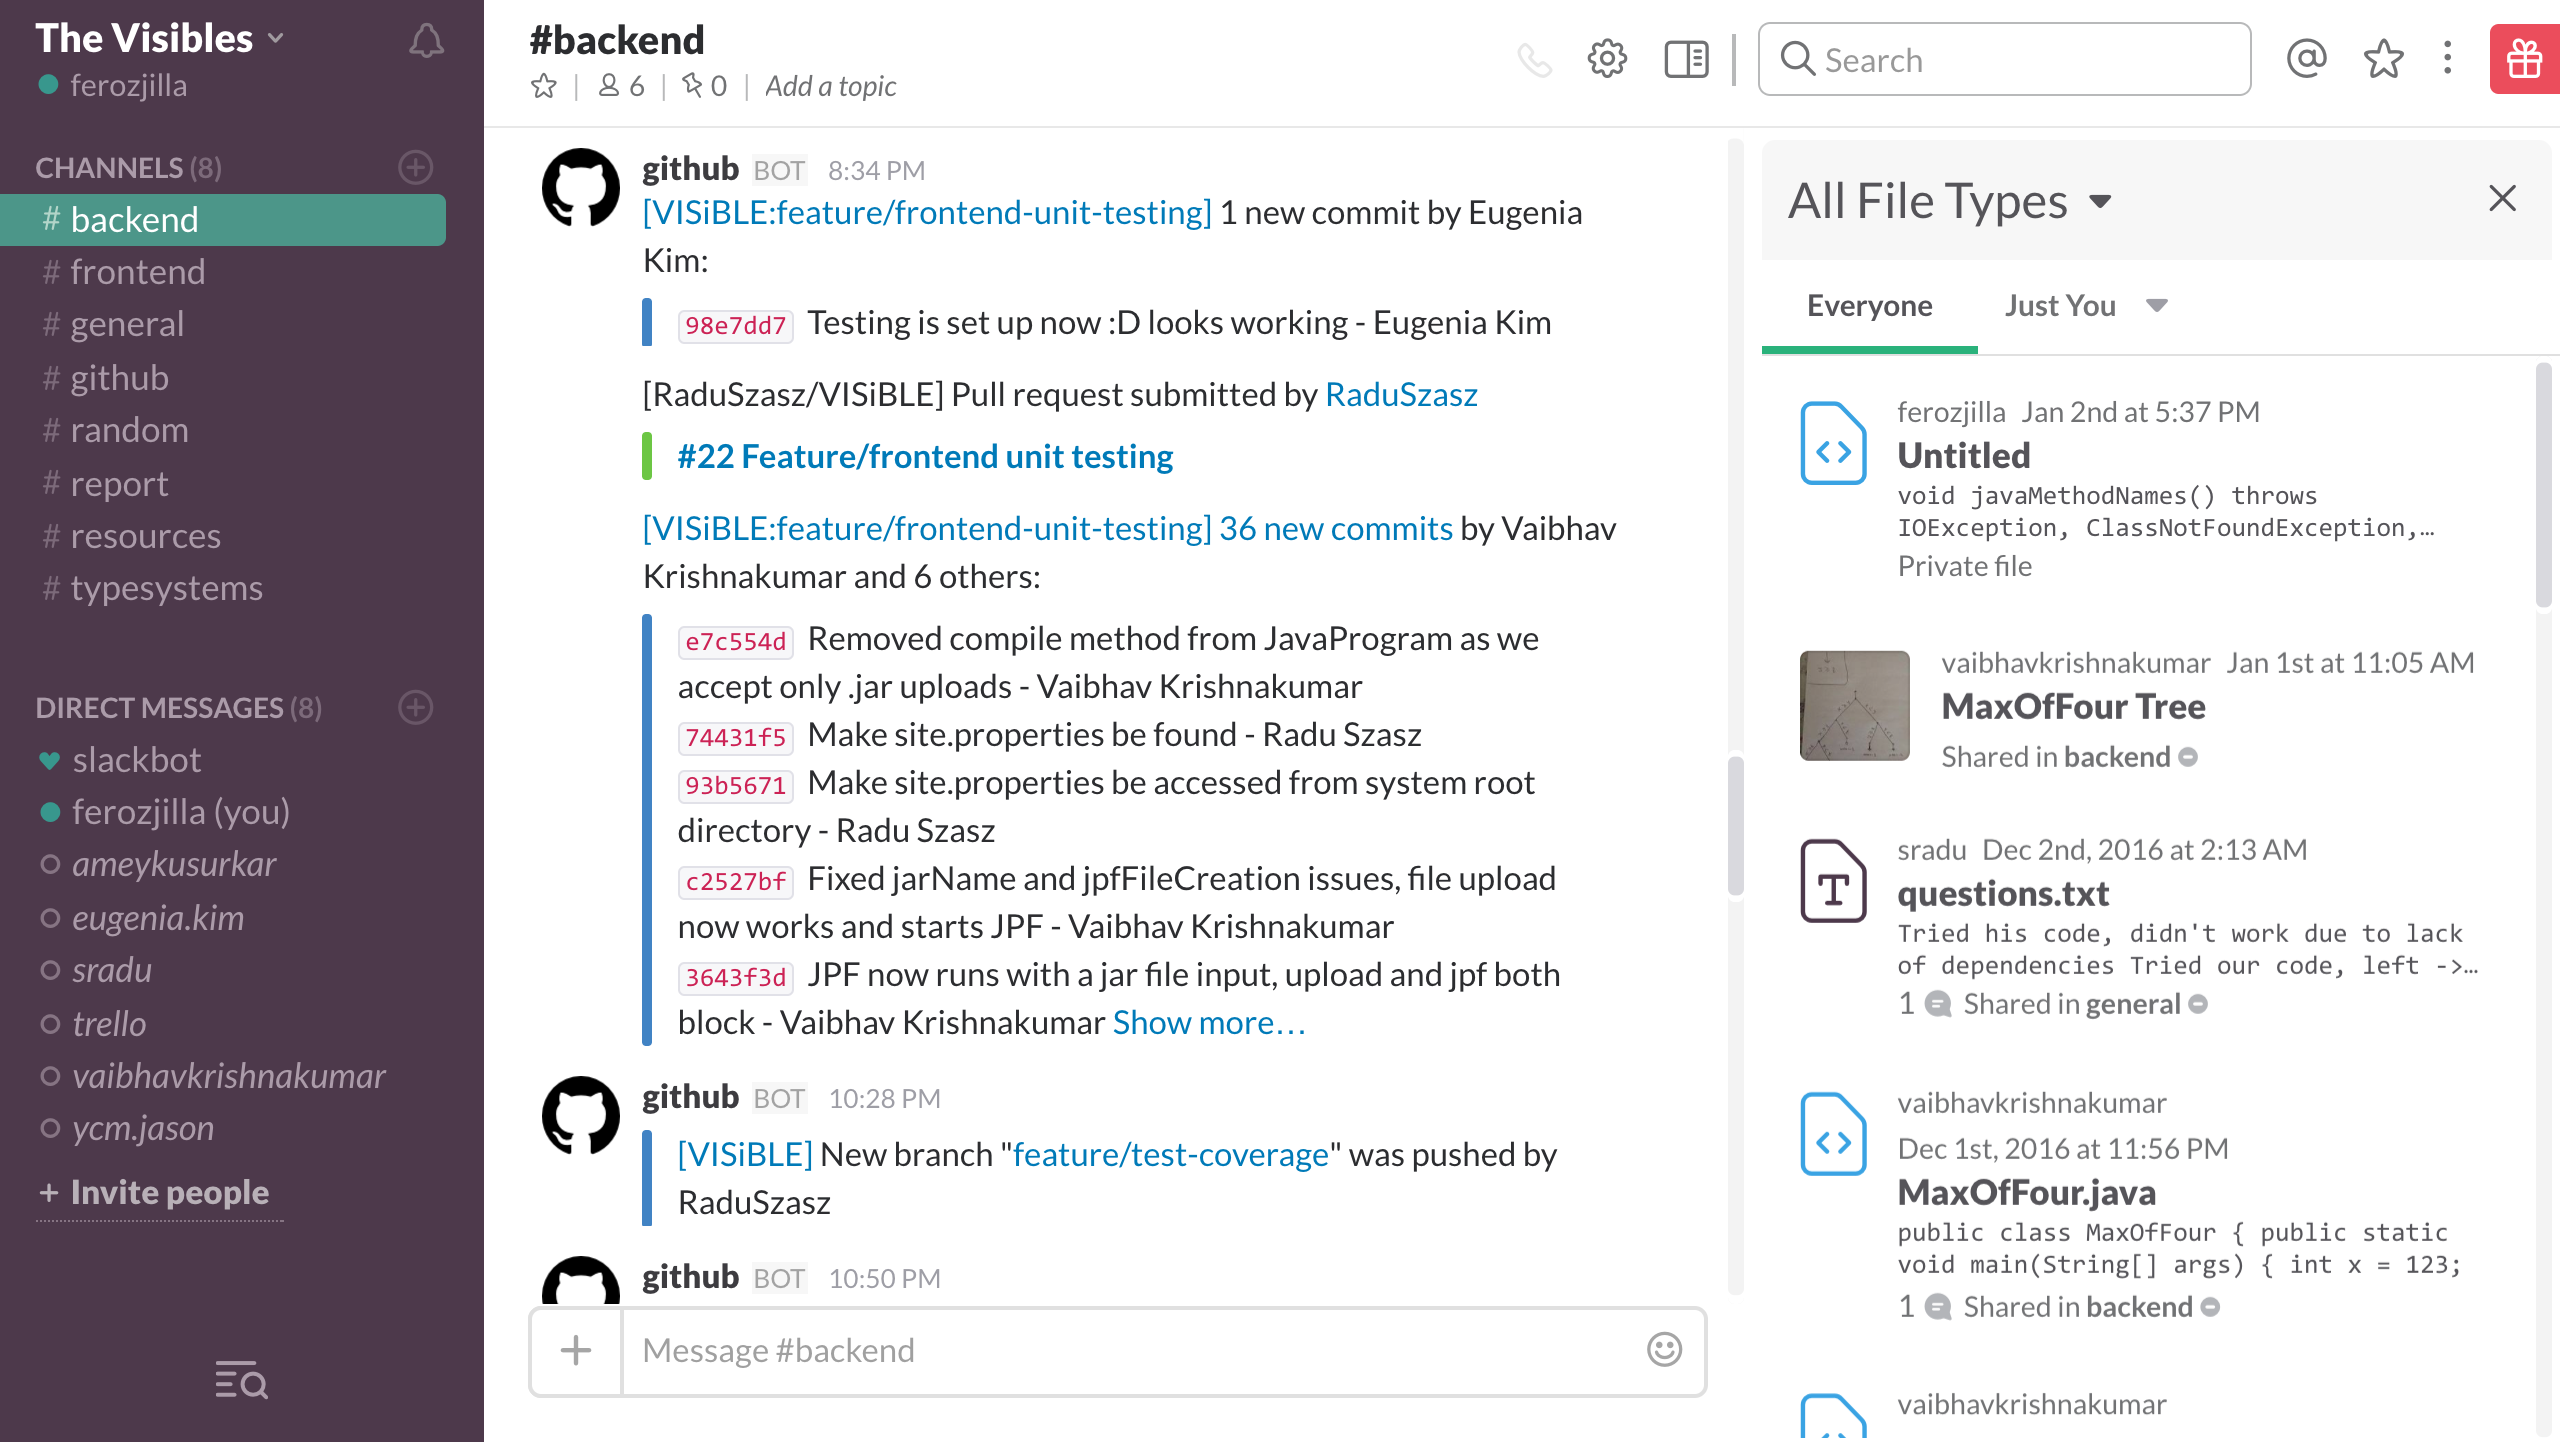
\includegraphics[scale=0.35]{slack.png}
\caption{Using Slack for effective resource sharing}
\label{fig:slack}
\end{figure}

\subsubsection{Communication}

During term time, across the iterations, we mostly worked as a group in labs, so most of the communication was done face-to-face, with everyone either individually approaching group members or addressing the group as a whole as needed. Besides face-to-face communication, we used mostly Slack \cite{slack}, Facebook Messenger \cite{messenger}, and Skype \cite{skype} as communication tools. \\

We found that each of the tools had their own strengths. We found Slack's channel-based communication to be very useful when the front-end and back-end teams wanted to communicate within themselves, without concerning the other team. Slack was especially convenient for sharing media and resources like web-links and source code files, which we might have constantly needed to refer to in the long run. We also used Slack when we quickly wanted to share blocks of code, as Slack's support for syntax highlighting made the code easy to read. What made Slack better than other messaging platforms for sharing content was the fact that the content could be easily found much later on. This can be seen in Figure \ref{fig:slack}, where all the files are neatly presented at the side even as the conversation moves forward. Also, as can be seen from the diagram, since we linked Slack with our GitHub repository, members were updated whenever someone one pushed code, making it easy to keep track of progress. \\

While Slack was very effective for sharing resources, we found that Facebook Messenger was much more effective for quick communication, and for addressing urgent issues. One of the main reasons was that due to the social aspects of Facebook Messenger, members checked their Messenger application for message updates much more frequently than Slack, making them more contactable via that platform. It was also easy to quickly ask questions on Messenger such as problems with understanding error messages, as we could simply take screenshots and pictures using the camera on our mobile phones. \\

These communication tools became especially necessary as we worked over the Christmas break, as all the group members were in different parts of the world for the holidays, and face-to-face communication was no longer possible. Communication between the front-end and back-end teams became key, as each team had to constantly update the other team regarding the updated format of inter-application communication as functionality evolved. This is when we found Skype invaluable for video conferencing. While we could not work simultaneously due to differing time zones, we used Skype to hold meetings and discuss plans, including updating our supervisor of our progress and clearing doubts with him.

\subsubsection{Management}

\textbf{Trello} \\

We found Trello \cite{trello} extremely useful for keeping track of the project's progress and task delegation. As mentioned earlier, the group was divided into a front-end and back-end team, with features internally divided into modular tasks which anyone in the team could work on. We had a Trello Board for each iteration with four sections, namely "To-Do", "In Progress", "Blocked", and "Finished", as can be seen in Figure \ref{fig:trello}. \\

At the start of each iteration, we would decide on a plan and break it down into tasks, which we would add into the "To-Do" section. The task cards were colour-coded to represent task categories such as front-end, back-end, integration, testing or miscellaneous. The colour-coding made it easy for members to find tasks that were relevant to them. Over the iteration, members would pick a task relevant to the team they were in, add their initials to the card and move it into the "In Progress" section. As we often did pair programming, both members' initials were reflected on the card. The card would then be moved into the "Finished" section after the task had been completed. If anyone got stuck on a task or ran into problems (as we often did with JPF), they would move the card into the "Blocked" section, and another group member who noticed that could then help out. A nice feature of Trello that we also utilised was the ability to comment on cards, which helped with the integration of the front-end and back-end. \\

\textbf{Travis CI} \\

Travis CI \cite{travis} is a continuous integration service that we used, by linking it to our GitHub repository. It provided us a hassle-free way to test our product as a whole. Whenever a member pushed new code to the GitHub repository, it would automatically build the project from scratch and run all the unit-testing and integration-testing modules, checking if the push was suitable for deployment. An advantage of this over running the tests locally was that Travis CI uses a fresh environment every time, preventing files and code from previous builds affecting the outcome of the test cases. Travis CI also proved invaluable in making collaboration more robust, as is explained later. \\

\textbf{GitHub} \\

The other major tool that we used was GitHub \cite{github}. The vast feature set of GitHub made it much easier for us to manage our code base and collaborate as a group. The branching functionality allowed us to keep a clear hierarchy and separation of concerns during the development process. The two main branches that were always present were \texttt{master} and \texttt{develop}. The idea was that \texttt{master} would always have a working product ready for deployment, and \texttt{develop} would have the most up-to-date code which was in development, but not necessarily ready for deployment. Hence, essentially \texttt{develop} was the "root" branch as far as development was concerned. Whenever a member or a pair would want to develop code, they would branch out from \texttt{develop} with a clear objective in mind for that branch, reflected in the name of the branch \cite{vincentdriessen2010}. \\

We followed the naming convention \texttt{feature/<feature-name>} for branches which aimed to implement features, and \texttt{bugfix/<issue-to-be-fixed>} for branches which aimed to fix issues. This made it easy to get get an idea of the state of the project just by looking at the names of the existing branches. When the objective of a branch was met, they would then merge their branch back into \texttt{develop}, and delete their branch. \\

However, to make the development process more robust, no one was allowed to simply merge their branch into \texttt{develop}. They had to make a pull request to \texttt{develop}, and pass two fail-safes before the branch could be successfully merged. Firstly, Travis CI would run all tests on the pushed code, requiring all the tests to pass. This ensured that the new changes did not break any old functionality. Secondly, the pull request had to be reviewed by another member of the group. This meant that someone else could check that the new changes were desirable, and check that the code followed good software engineering principles. It also allowed the rest of the group to stay updated on what the other members in the group were doing. Only after the tests passed and another member approved the changes, was the branch allowed to be merged into \texttt{develop}. \\

\textbf{Postman} \\

Postman \cite{postman} provides an interactive graphical interface to make HTTP requests, making it easy to define request parameters and visualise the response. As the back-end was developed independently from the front-end, this tool proved to be very useful to test the end points of our application. It allowed us to simulate the front-end and see how it would interact with the back-end, in order to verify that the back-end responded as expected. The ability to quickly and efficiently change request parameters and simulate requests without a browser helped our productivity hugely.

\begin{figure}
\centering
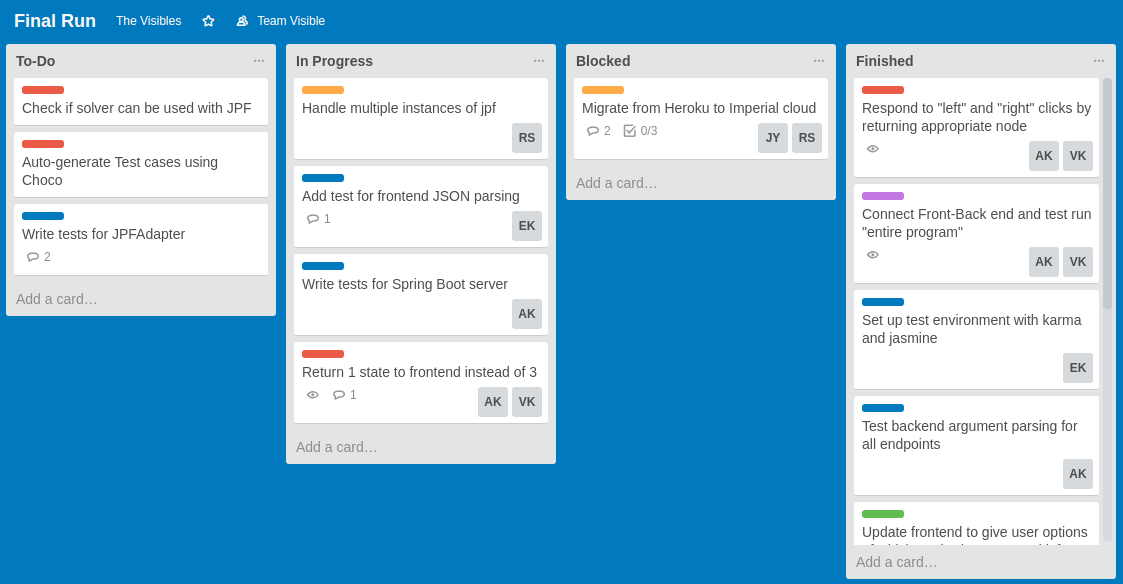
\includegraphics[scale=0.45]{trello.png}
\caption{Screenshot of Trello Board}
\label{fig:trello}
\end{figure}

\section{Design and Implementation}

As mentioned above, the structure of our project allowed a clear separation of concerns. We efficiently developed the two halves of our project independently: the front-end - an Angular2 application which dealt with visualisation of data and user interaction; and the back-end - a Spring Boot application which handled requests and interacted with the JPF library. We will describe the two sections independently, dedicating one section on how we glued them together.

\subsection{Integration}

\subsubsection{Building}

While we aimed for low coupling among the different elements of our project, in certain situations we wanted the components to act cohesively. \\

One such situation is the build process. We found it vital to run a single command to build all the parts of our project. The tool we chose to help us pursue our goal is Gradle \cite{gradle}. It provided us with vast amounts of online resources, plenty of plugins for the technologies we were using throughout our project, integration with Travis CI and the ability to configure our custom tasks, may it be the case we need it. \\

The plugins mentioned were vital in saving us valuable time. Without them, we would have reinvented the wheel multiple times while setting up our project. \\

The configuration of our build was similar to the organisation of our project. We split into two distinct subprojects which had their build.gradle files, describing their build. \\

When the "build" task came to an end, an end-to-end working app resulted. And it's not just the building that this task handled. Our tests were run on every invocation, to make sure that the newly produced version of our application will not have obvious flaws. \\

\subsubsection{Communication Protocol (a.k.a. the API)}

Agreeing on a communication protocol was essential for seamless integration into one working product. \\

We valued keeping the API used as well documented and clear as possible. We used Swagger \cite{swagger} to create an interactive interface which allowed us to try our endpoints immediately, as well as describe them to any newcomer wanting to make an impact in our project - essential given our desire to open source our project. This generated page stands as the best description of our communication protocol and its vital components are presented in Figures \ref{fig:upload}, \ref{fig:symbolicmethod} and \ref{fig:step}. 

\begin{figure}
\centering
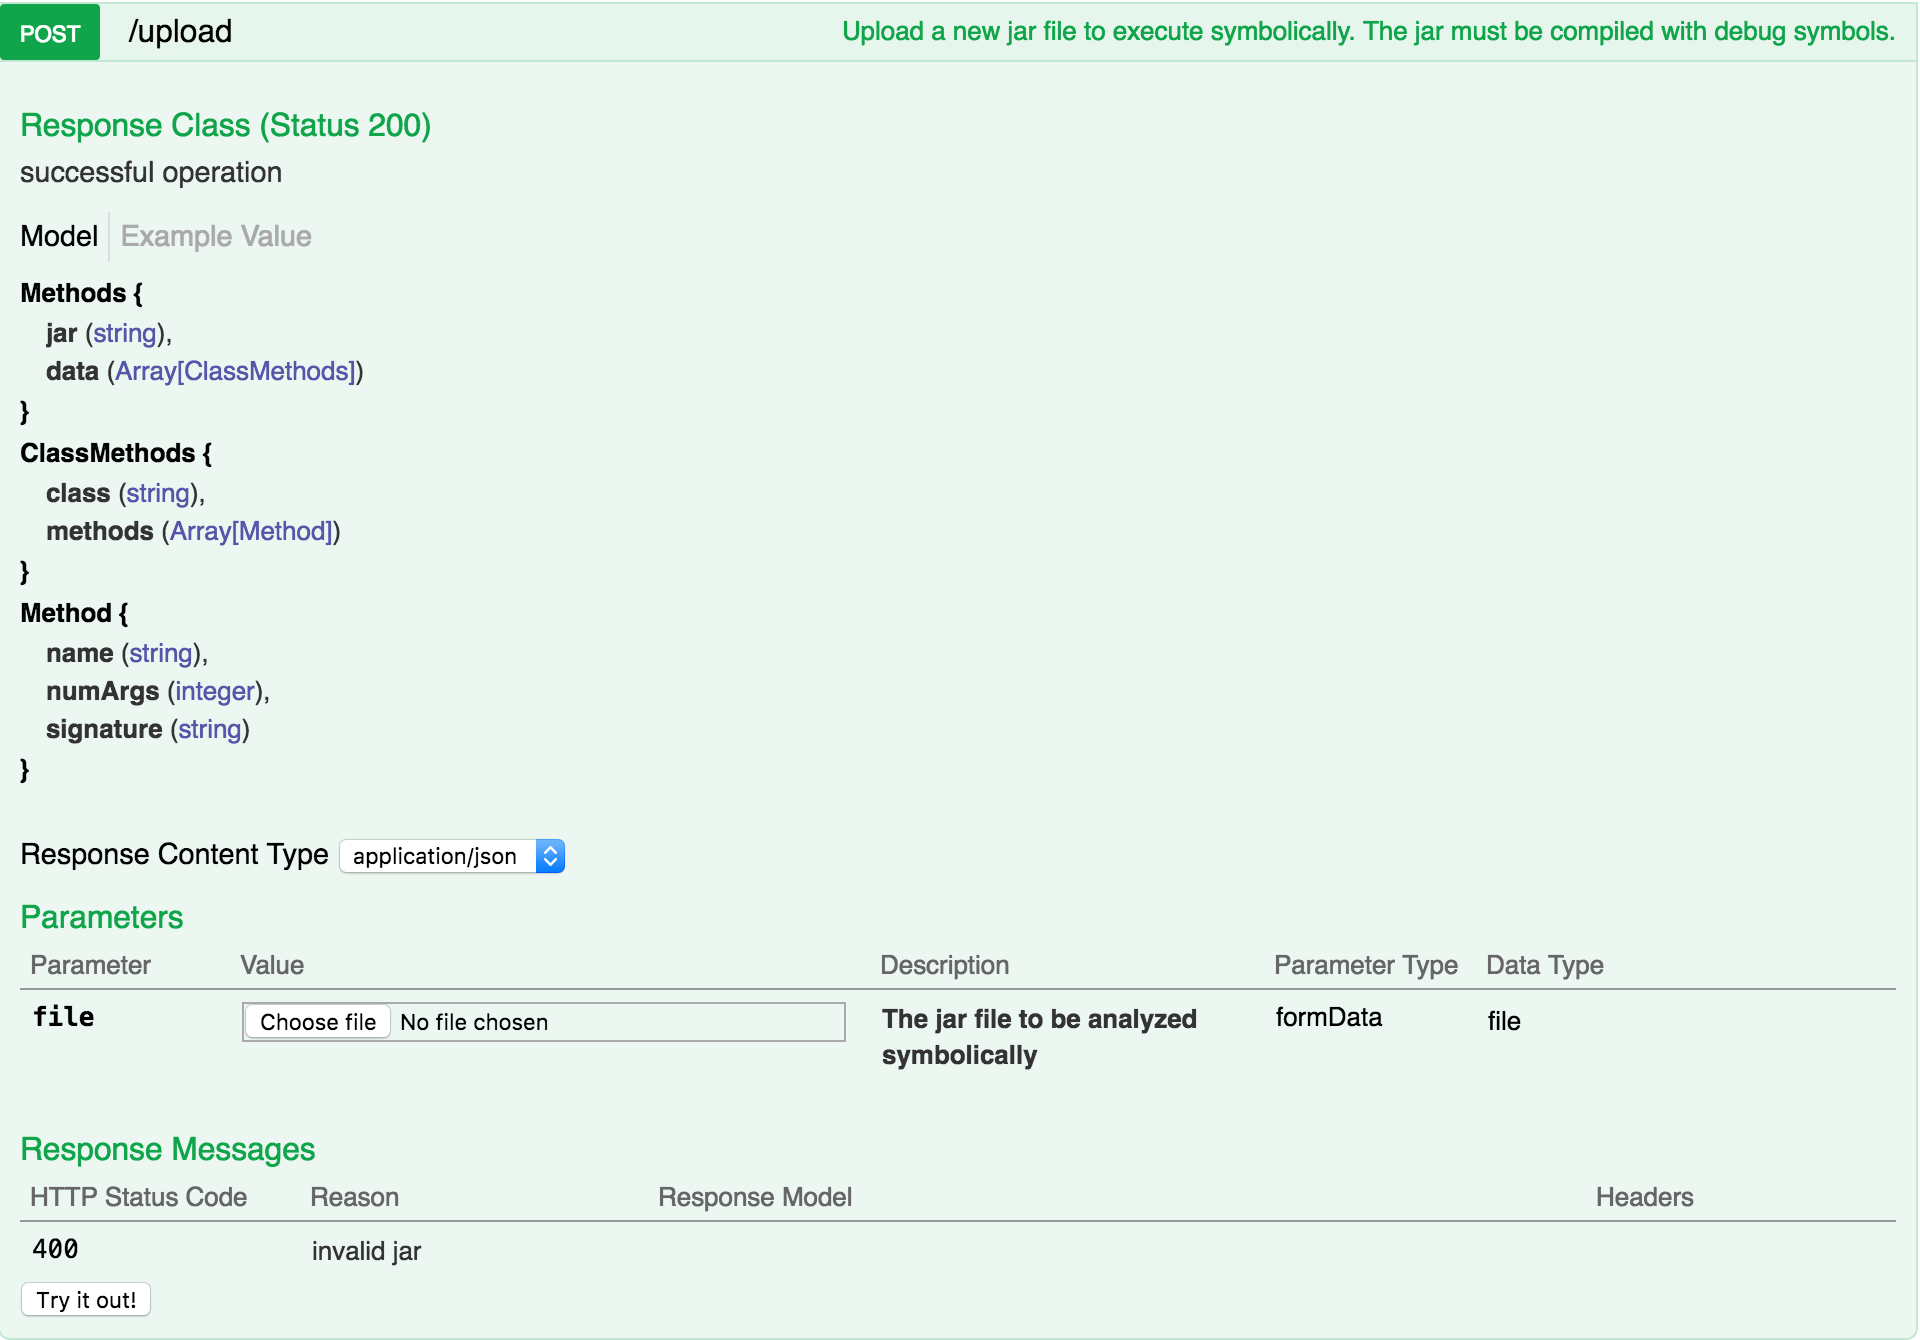
\includegraphics[width=450pt, height=270pt]{upload_controller.png}
\caption{The description of the \texttt{/upload} endpoint}
\label{fig:upload}
\end{figure}

\begin{figure}
\centering
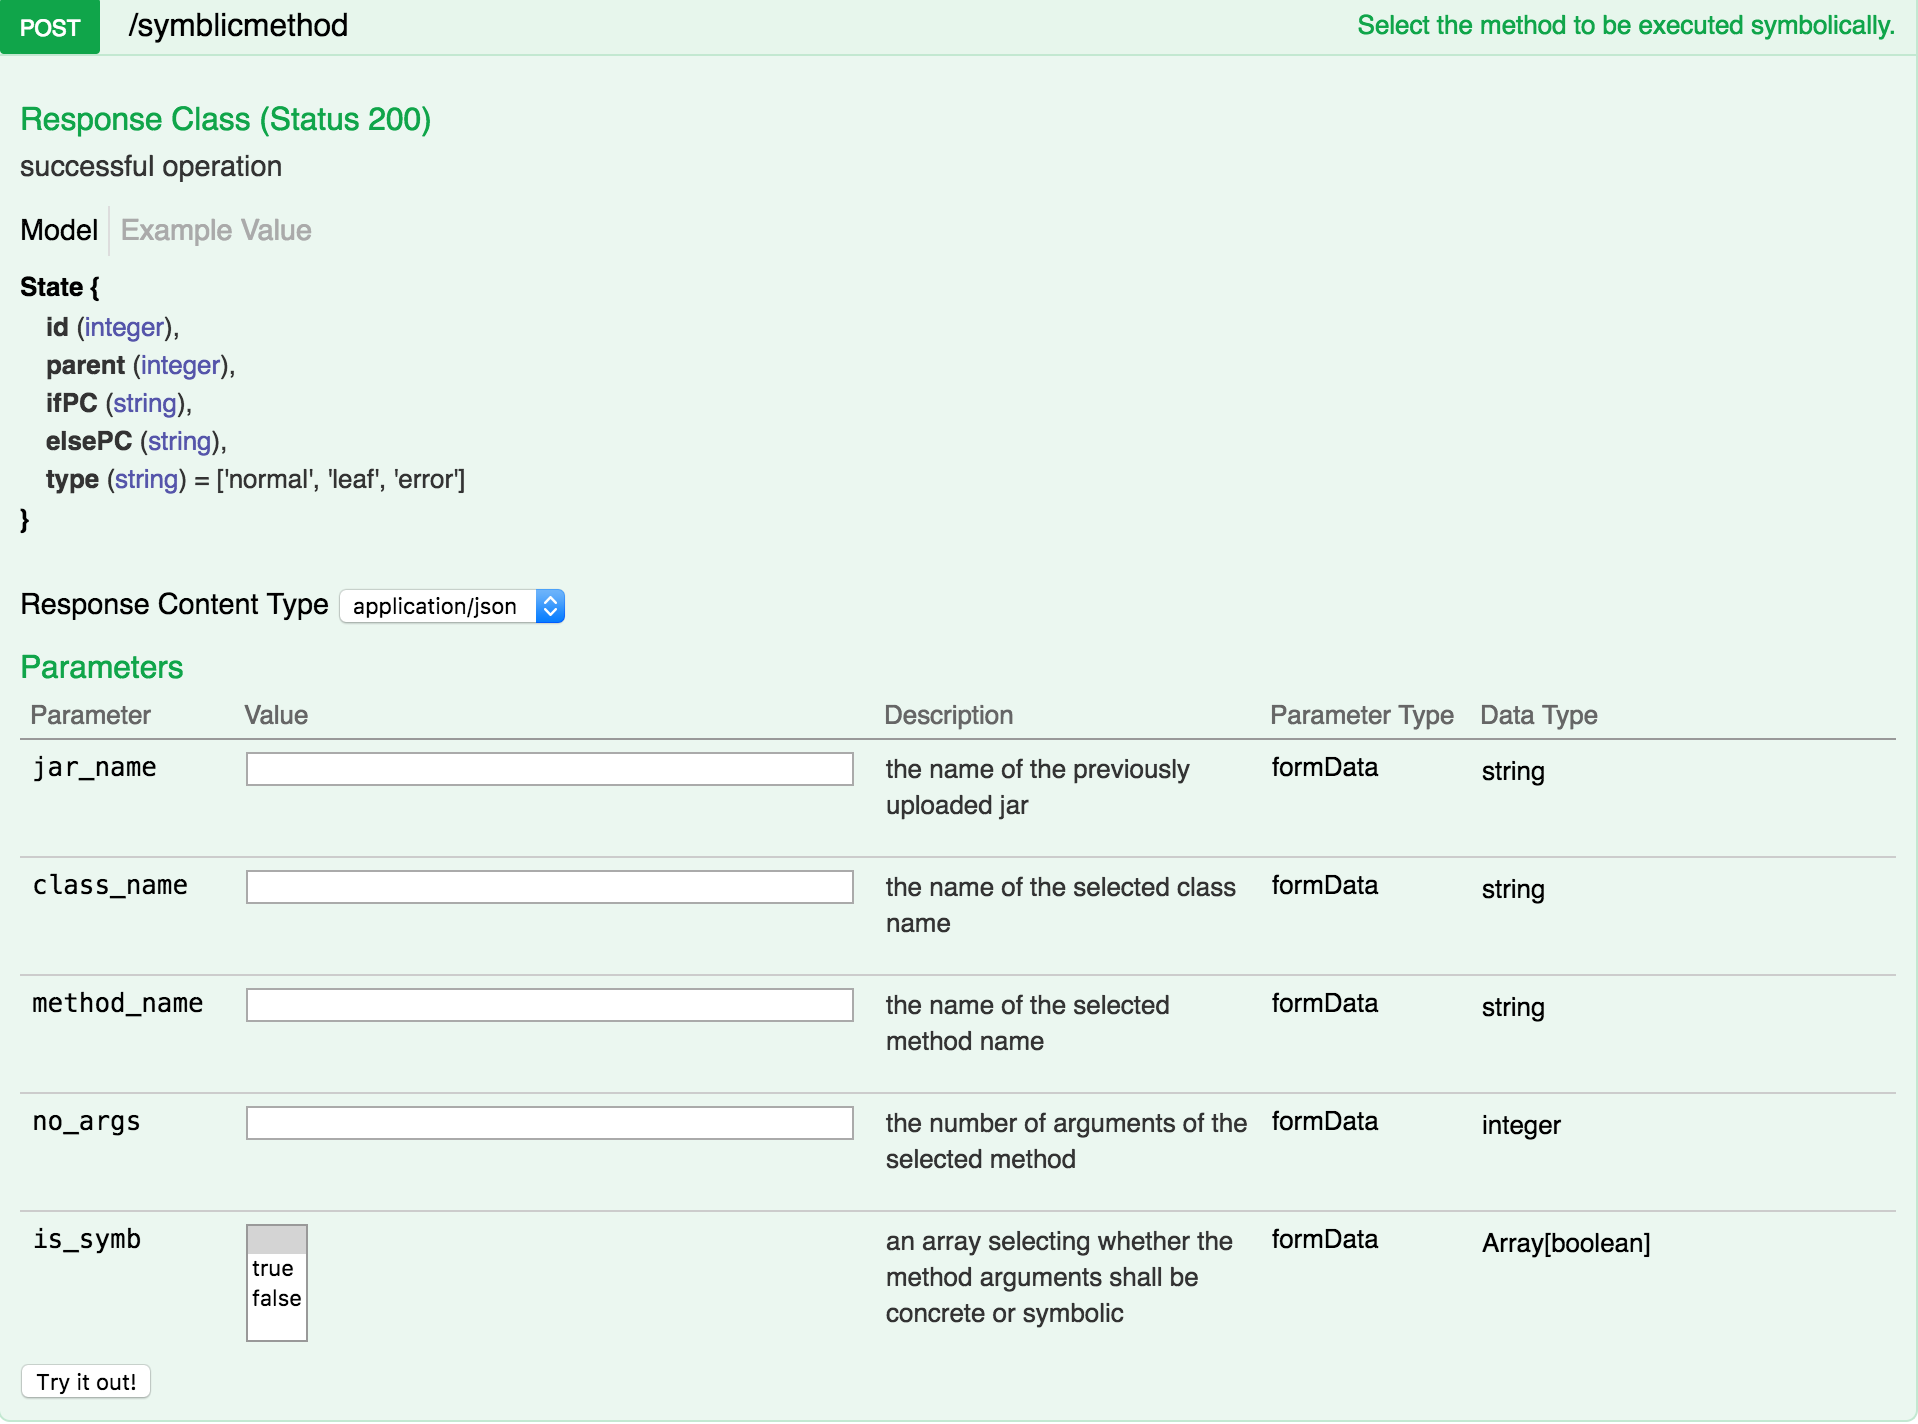
\includegraphics[width=450pt, height=270pt]{symbolic_method_controller.png}
\caption{The description of the \texttt{/symbolicmethod} endpoint}
\label{fig:symbolicmethod}
\end{figure}

\begin{figure}
\centering
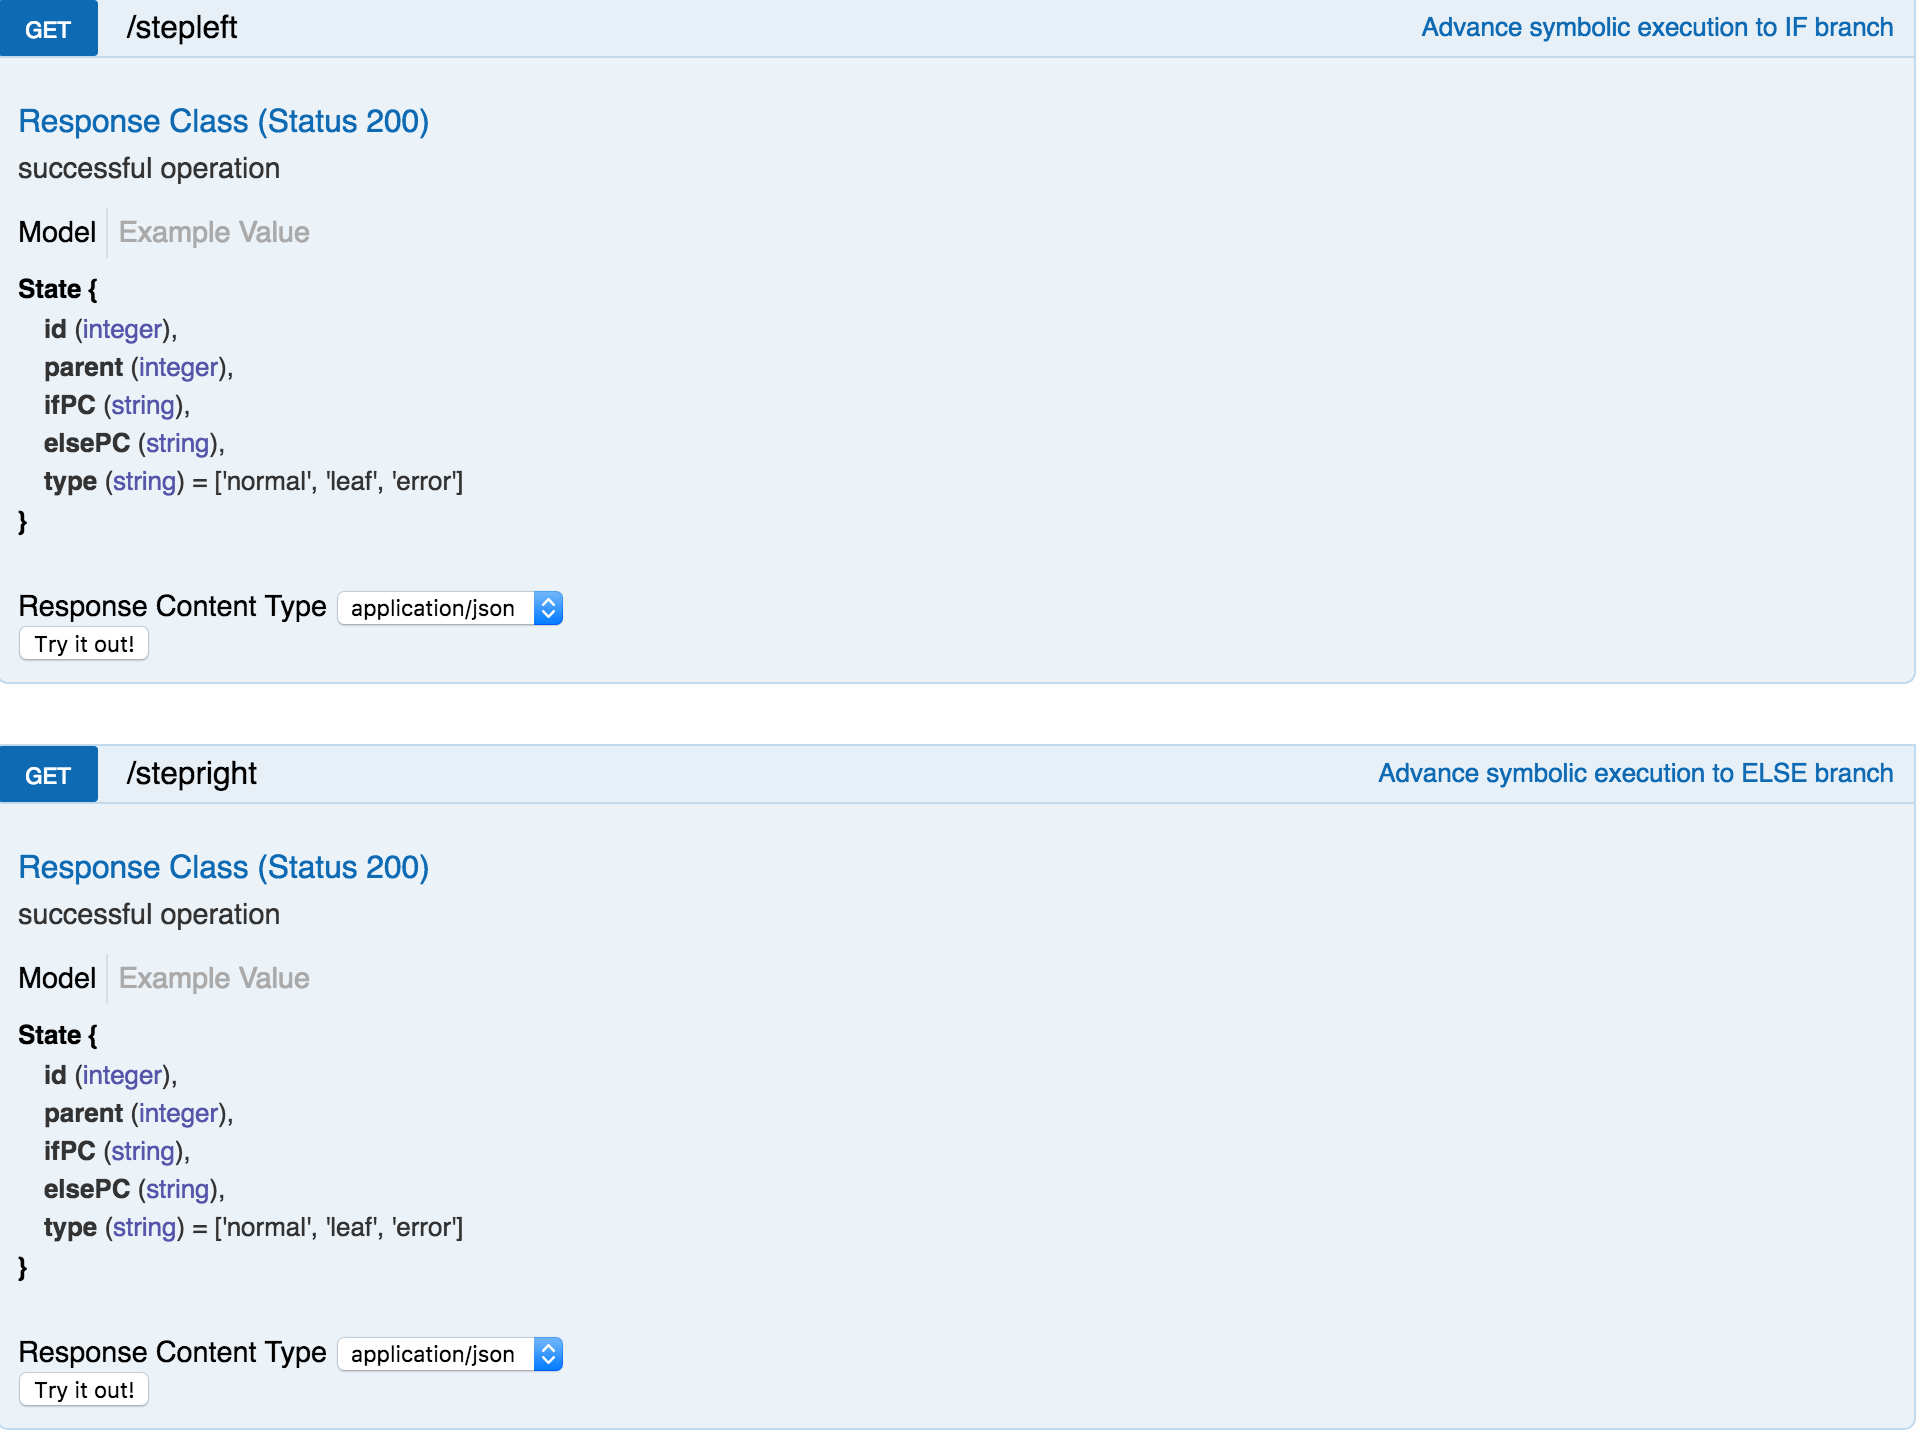
\includegraphics[width=380pt]{step_controller.png}
\caption{The description of the \texttt{/stepleft} and \texttt{/stepright} endpoints}
\label{fig:step}
\end{figure}

\subsection{Back-end}
The back-end for VISiBLE is further split into two, fairly distinct parts. One part is the Spring Boot application which handles requests from the front-end and co-ordinates the different components of the back-end, including the \texttt{SymbolicExecutor}, which it treats as a black box. The \texttt{SymbolicExecutor} essentially provides a simple interface to allow external control of the execution path of a Java Program by internally feeding it to JPF and interacting with it.

\subsubsection{Spring Boot Application}

\paragraph{Why Spring Boot?}

Since our project revolved heavily around the JPF libraries, which were written in Java, our back-end had to be written in Java to utilise these libraries. Naturally, it made sense to use a Java application framework. This immediately eliminated many commonly used web application frameworks such as NodeJS and Ruby on Rails, due to language constraints. \\

We felt that Spring Boot, which builds web applications using the Spring Application Framework, was the go-to Java Framework for us for several reasons. The framework was easy to set-up, requiring minimal configuration. It has very good documentation and a large community, which made it easy to pick up. It also has other useful features such as easy-to-configure dependency injection and an extensive testing framework. The framework also makes it easy to introduce routing into our back-end web service, using decorators to map classes and methods to end points. On top of all this, some of the group members had previous experience with the framework, helping us to eliminate the initial time spend on getting used to a new framework.

\paragraph{Application Overview}

The Visible Server Application essentially aims to co-ordinate the different components in the back-end and serve front-end requests. Through four end points, the back-end provides an API to upload a Java Program, choose a method for \texttt{SymbolicExecutor} to run symbolically, and steer the execution path of the program. This process is summarised in Figure \ref{fig:visibleserver}. \\

\begin{figure}
\centering
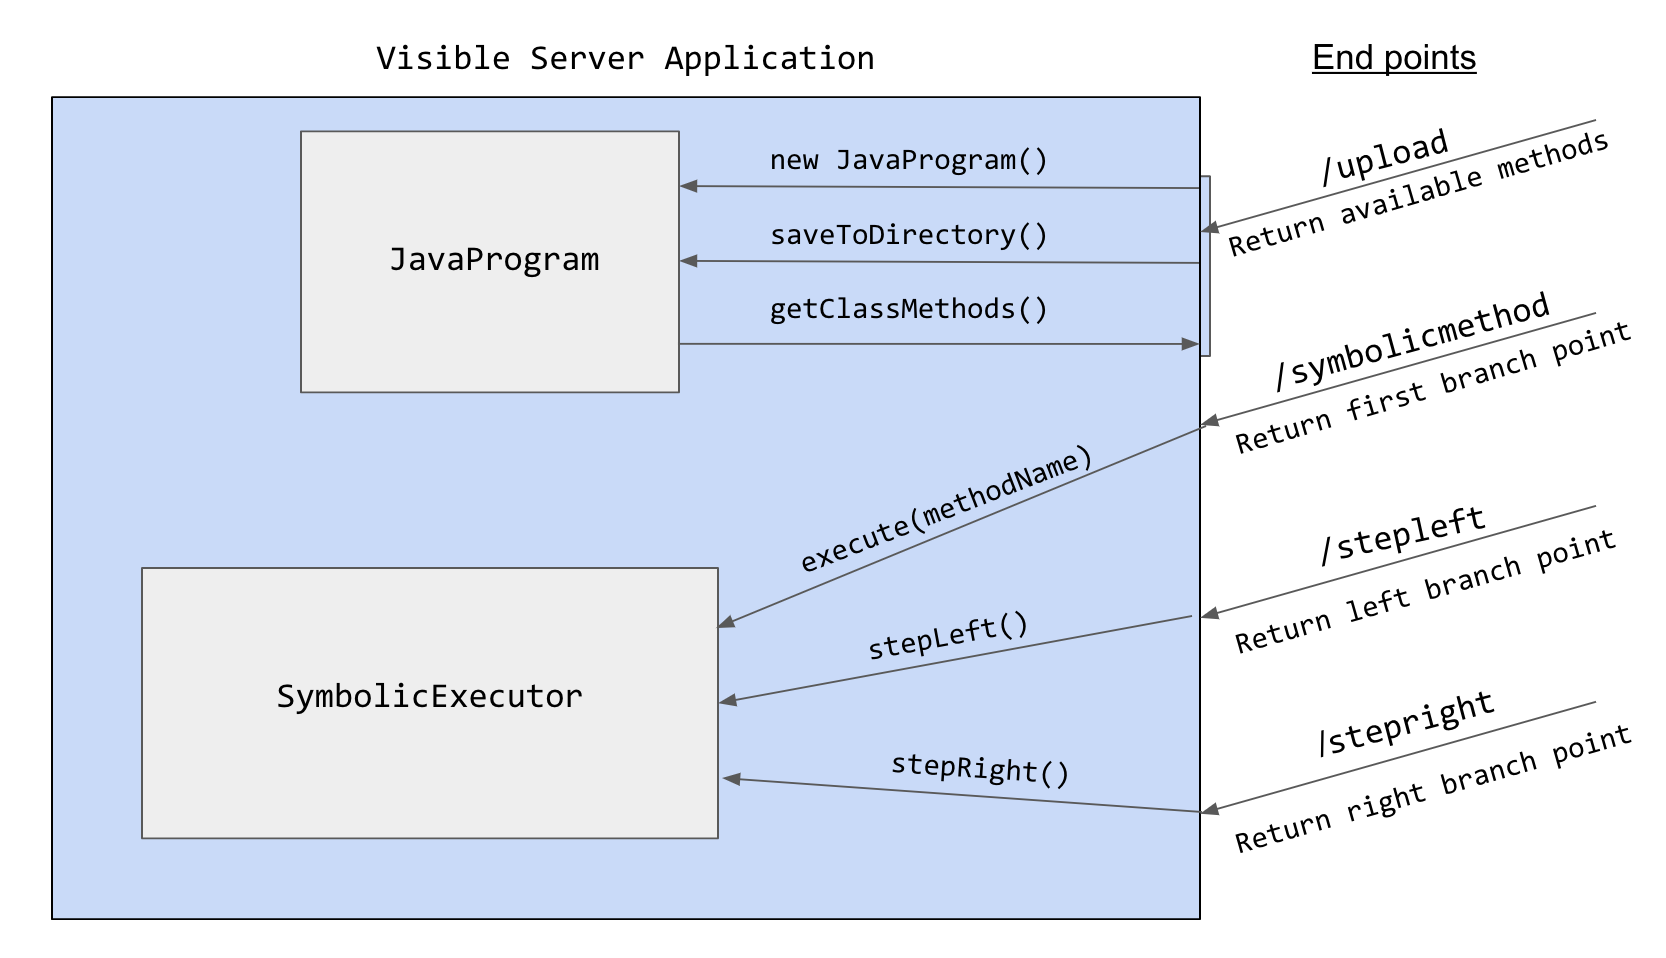
\includegraphics[scale=0.45]{visibleserver.png}
\caption{Back-end architecture overview}
\label{fig:visibleserver}
\end{figure}

The back-end receives a \texttt{jar} file to execute through a POST request to \texttt{/upload}. The file data is then passed into \texttt{JavaProgram}, a class which encapsulates a Java program and provides methods to handle operations relating to the program. \texttt{JavaProgram} handles two main jobs. Firstly, it saves the \texttt{jar} file to disk in the correct directory, where \texttt{SymbolicExecutor} will later look for it. Secondly, it reads the \texttt{jar} to find all the classes and methods in those classes, and extracts the relevant method data. This is done so that the back-end can respond with all the possible methods in the \texttt{jar} which can be run symbolically. This data is encapsulated within a \texttt{ClassMethods} object, and \texttt{JSON} serialised before being returned (an example response \texttt{JSON} object is shown in Figure \ref{fig:methodsjson}). This operation is made easy using the Java standard library classes \texttt{Class} and \texttt{Method}, from which information can be extracted. The two operations are accessed using the methods \texttt{saveToDirectory()} and \texttt{getClassMethods()} respectively. \\

\begin{figure}
\centering
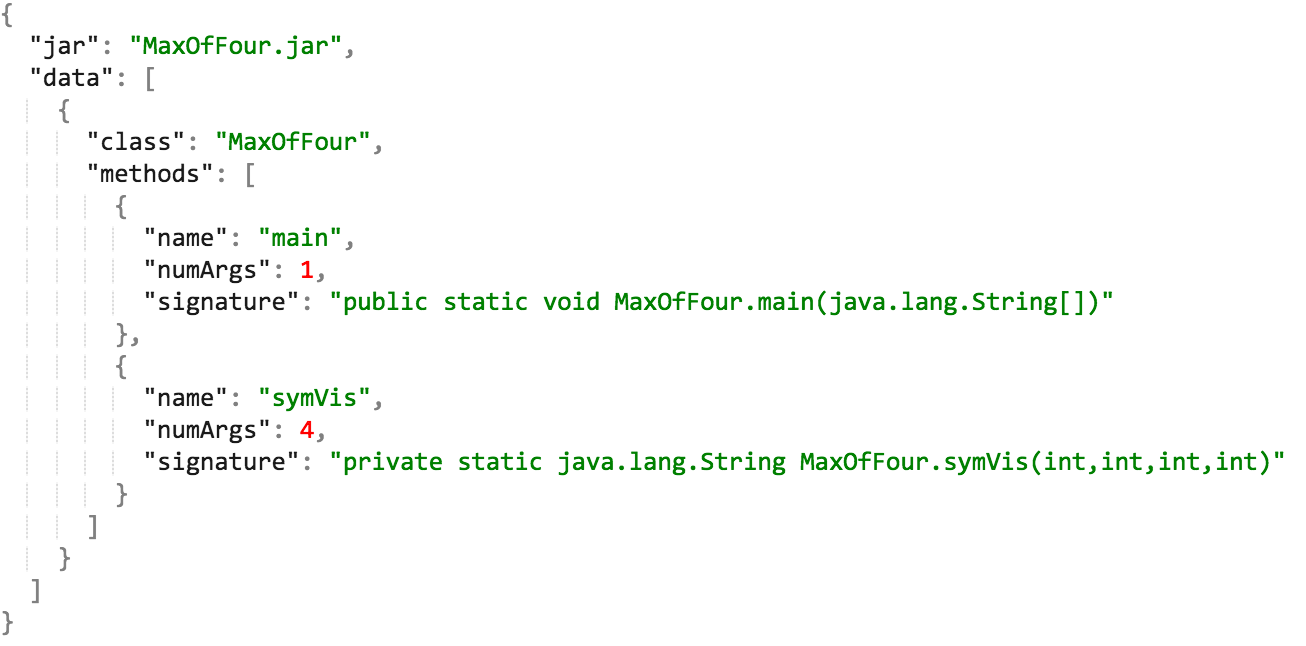
\includegraphics[scale=0.6]{methodsjson.png}
\caption{A JSON response with Java methods and corresponding data}
\label{fig:methodsjson}
\end{figure}

The back-end can then be requested to execute the uploaded \texttt{jar} file with a POST request to \texttt{/symbolicmethod}, with parameters specifying which method to be run symbolically, and which of the arguments to the method should be symbolic. With this information, the application can then ask \texttt{SymbolicExecutor} to start running. The \texttt{SymbolicExecutor} returns the first \texttt{State} in the execution. \texttt{State} encapsulates a branching node in the execution path of the program, where a binary decision can be made to go either "left" or "right". As with \texttt{ClassMethods}, the \texttt{State} is serialised into JSON before being returned (as shown in Figure \ref{fig:statejson}). \\

\begin{figure}
\centering
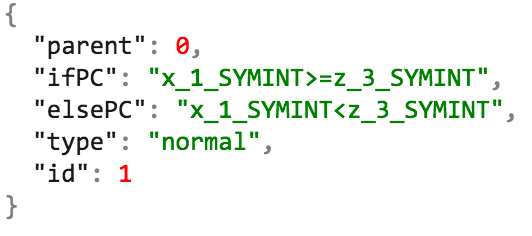
\includegraphics[scale=0.7]{statejson.png}
\caption{A JSON response representing a node in the execution tree}
\label{fig:statejson}
\end{figure}

Once the \texttt{jar} file has been uploaded and symbolic method chosen, the back-end then allows the execution of the Java program to be steered left or right at binary decision points through the GET requests to \texttt{/stepleft} and \texttt{/stepright} respectively. The application then interacts with \texttt{SymbolicExecutor} by calling either \texttt{stepLeft()} or \texttt{stepRight()}, which return the \texttt{State} corresponding to the next branching point down the execution path chosen. \\

\paragraph{End-point Routing}

Spring Boot makes it very easy to set-up end points for the application using decorators. Essentially, we create controller classes to manage end points and then define methods to handle requests. For example, adding the \texttt{@RestController} decorator to a class informs Spring that it is going to be used as a controller. We can then simply add \texttt{@RequestMapping("/<end-point>")} to a method in the controller, and that method will be called whenever \texttt{/<end-point>} is accessed. Subsequently, we can also add decorators like \texttt{@PostMapping} to define the type of request the method handles. \\

Spring Boot also makes it easy to access the request's parameters, as Spring will pass them into the method if the arguments have \texttt{@RequestParam} decorators. For example, in \texttt{FileUploadController}, the method that handles file uploads has the signature:  
\[ \texttt{handleFileUpload(@RequestParam("file") MultipartFile file, ...)} \]
Spring takes the uploaded file in the request, puts it together and passes it into the method as an argument, which can then be used in the method as a Spring \texttt{MultipartFile} object, which supports regular file operations. Hence, on the back-end, we never have to leave the Java programming context even when dealing with HTTP requests, truly treating it as an abstraction. This structure also makes it easy to separate the concerns of the various end points into different classes. 

\paragraph{Serialising Objects using Jackson}

In our back-end design, we used classes such as \texttt{ClassMethods}, \texttt{MethodData}, and \texttt{State} to build and encapsulate data that would be returned from a HTTP request. One reason for this design choice was the ease and versatility with which the Jackson library can serialise Java objects into JSON objects. By default, when given a Java object, Jackson \cite{jackson} can automatically take the fields in the class and produce a JSON object with minimal configuration. The \texttt{toString()} methods of these classes were then overridden to return a string representation of the object in JSON notation. \\

However, the strength of Jackson lies in the customisability of the serialisation. We added decorators like \texttt{@JsonInclude(JsonInclude.Include.NON\_EMPTY)} to the error message field to only include it in the JSON if there was an error. We could also extend \texttt{JSONSerializer} to define our own serializers for classes or fields that needed to be serialised in a custom way. This was helpful when \texttt{ClassMethods} needed to be serialised as a list of key-value pairs instead of the default object-with-fields approach, and when the \texttt{parent} field of \texttt{State} (which in turn is another \texttt{State}) needed to be serialised as just its id, instead of the \texttt{State} itself.

\subsubsection{Symbolic Executor}
The use of the symbolic executor is an example of the Adapter design pattern in use. This gives us one key benefit - we do not exclusively rely on JPF as part of our application. In theory, \textit{any} program which is capable of navigating the program tree and returning the suitable nodes can be used in the executor. The removal of this dependency makes VISiBLE much easier to extend; in addition, we can isolate testing of JPF from the testing of the executor via the use of mock objects. \\

For VISiBLE, JPF was used as the symbolic executor to navigate the program tree. The configuration of JPF is a long and tedious process but worthwhile for the benefits that it produces. As a result, despite what we had initially assumed, JPF is \textit{not} a black-box for us - we needed to know it's internal structure and methods to use it effectively. We explain the workings of JPF briefly in the following sections for completeness; much of this understanding comes from the JPF-Wiki \cite{corinapasareanu2016} and the knowledge of our supervisor, who is one of the developers of the latest version of JPF. 

\paragraph{What is JPF?}
JPF - or Java Path Finder - is a virtual machine for Java bytecode written and released by the Ames Research Center, a part of the US Government's space initiative NASA. It is designed as a highly extensible application, with the core utility \texttt{jpf-core} providing simple model checking and verification capabilities. Much of our computation in JPF was performed by the external module \texttt{jpf-symbc} - this provides symbolic execution and path condition generation in addition to the features provided by the core utility. \\  

JPF is written entirely in Java. Thus, it is a VM running atop the standard JVM. However, unlike the standard JVM, JPF runs the Java program by executing \textit{all possible} paths through the program. This provides significantly more information with the trade-off being a higher execution time. JPF is not a lightweight tool and can be customised to fit a variety of purposes.   

\paragraph{How does it work?}
Much of the early part of our project involved working out the internals of JPF. The documentation is very limited, with the existing user pool being a small number of people using JPF for very specific purposes. With this limited help and the support of our supervisor, we understood the basics of JPF's execution of a given Java program. \\

The Java program interacts with JPF via listeners, classes which contain a variety of methods called by JPF as part of its execution. This follows the event-driven programming paradigm, where each action performed by JPF results in a function being called in the listener. The listener provides hook methods which can be overridden via custom implementations to react to the events as necessary. Methods in the listener include \texttt{stateAdvanced()}, \texttt{stateProcessed()}, \texttt{searchFinished()} and \texttt{stateBacktracked()}. \\

JPF keeps track of program execution using a \texttt{Search} class which represents JPF's traversal through the program. This holds valuable information such as the point along program execution we are currently at, the instruction being executed and details on the current thread which is executing. JPF also stores information about program execution at a particular point using \texttt{SystemState}s. This contains data which allows us to reconstruct the snapshot of the VM at that instant, a useful way to implement re-storable states. \\

Furthermore, at every decision point in the program, JPF generates a \texttt{ChoiceGenerator}; this key component allows us to pick which execution path to follow based on different criteria. As an example, decisions include which thread to run at a context switch or which branch of an \texttt{if} statement to follow. Methods in the listener are called every time we advance \texttt{SystemState} or \texttt{ChoiceGenerator}.

 \paragraph{How does VISiBLE use JPF?} 
Frustratingly, while JPF does provide API to work with (The Verify API \cite{verify}), it requires Java program to have special JPF annotations. Since the primary purpose of our project was to run JPF on an arbitrary Java program, this was not an option for us. Thus we had to write our own mechanism for interacting with JPF. \\

Given the interactive nature of VISiBLE, we had to block and resume JPF at multiple points along the execution. Since our supervisor had informed us that JPF was not thread-safe, and JPF ran concurrently with other threads in our application, we foresaw potential concurrency issues. We mitigated this risk via the introduction of synchronisation mechanisms such as latches. \\

\begin{figure}
\centering
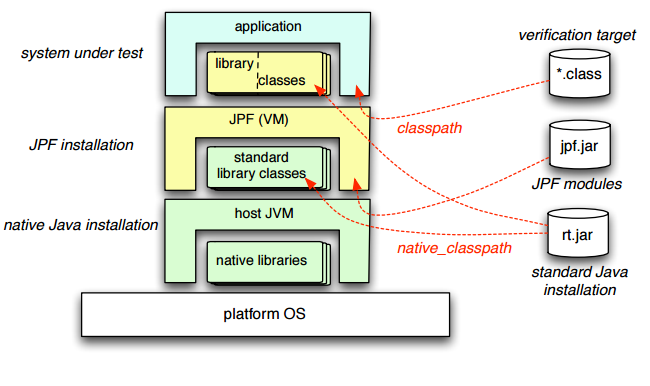
\includegraphics[scale=0.4]{jvm_jpf_overview.png}
\caption{JPF Architecture Structure - VISiBLE lies between JPF and the system-under-test \cite{petermehlitz2010}}
\label{jpf_jvm}
\end{figure}

Since our knowledge of JPF's inner workings was fairly basic, we designed a simple mechanism to interact with it. This involved two parts - the \texttt{JPFAdapter} which configures and executes JPF, and \texttt{VisualiserListener}, our extension of JPF's listener. Figure \ref{jpf_jvm} shows the structure of JPF by itself - VISiBLE is an application between the system-under-test and JPF, providing the extra functionalities mentioned earlier. 

\begin{figure}
\centering
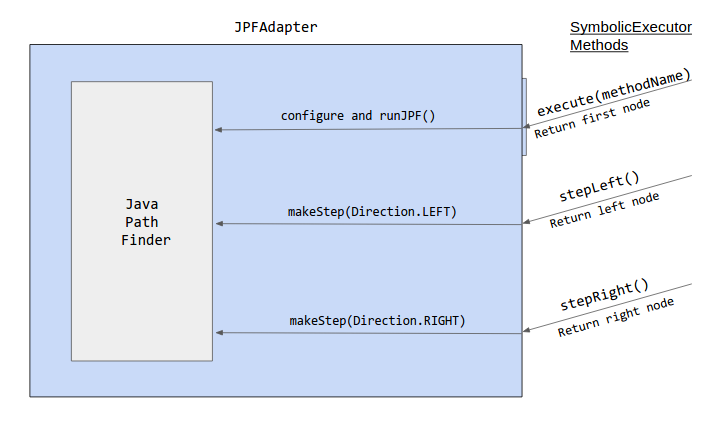
\includegraphics[scale=0.6]{adapter.png}
\caption{\texttt{JPFAdapter}, implements \texttt{SymbolicExecutor}} 
\end{figure}

\subparagraph*{\textbf{JPF Adapter}}\mbox{}\\

The \texttt{JPFAdapter} provides a further level of encapsulation within our application. It implements the \texttt{SymbolicExecutor} interface and is used to configure and execute JPF. This turned out to be a challenging part of the project due to the complexity of configuring JPF. Creating the \texttt{config} file, a set of key-value pairs, involved the use of hard-coded file paths which had to be abstracted out of our code. In particular, the \texttt{site.properties} file is machine-specific and contains an absolute file path to the source code of \texttt{jpf-core}. This made collaboration and deployment especially difficult as we had to remember to change the configuration to match our machine. \\

The constructor to the adapter takes in all the information that we need to configure JPF. The user provides a \texttt{jar} file whose name we store; using this and the Java \texttt{JarFile} class, we can get access to the \texttt{Manifest} and the name of the class with the \texttt{main} method. Furthermore, we need the names of the method that the user executes symbolically, and the class it belongs to. A feature we added later was to allow mixed concrete and symbolic (so called "concolic") inputs. Thus, we store a boolean array which denotes whether each argument is symbolic or not. \\

These parameters are processed internally by the adapter, creating the key-value pairs that are then put in the \texttt{config} file. JPF provides a \texttt{Config} class that allows us to do this neatly, without having to explicitly write to a file. The final piece of configuration is to instantiate our listener - this has to be added explicitly as JPF uses the built-in \texttt{SymbolicListener} by default. We will explain the role of the listener in further detail in the next section. \\

Having completed the set-up, the adapter runs JPF via an \texttt{ExecutorService}; as mentioned earlier, JPF is not a lightweight application. While JPF is being initialised, we do not want any calls to the \texttt{SymbolicExecutor}. We use a \texttt{CountdownLatch} to deal with this concurrency problem. This behaves as a binary semaphore, blocking the main thread until we receive confirmation that JPF has successfully initialised. \\

Upon initialisation, the adapter automatically returns the first node to the callee. This is the first branching point in the user program. For subsequent calls, the adapter's \texttt{makeStep(direction)} method is used to steer program execution. The \texttt{direction} parameter is passed on to the listener which deals with moving forward on the correct branch of the given node. Once the Java program has finished execution, the adapter is in charge of terminating JPF and informing the server of the final state. \\

Error-handling is made difficult by the fact that JPF internally deals with errors as part of its execution - after all, it is built for model-checking and verification. For such cases, we simply inform the front-end that an internal error occurred in JPF. Any errors in the \texttt{JPFAdapter} are dealt with in a nicer way - since our final output to the front-end is a \texttt{State}, we create an optional error field as part of our representation. The JSON Serialiser mentioned earlier adds this error message only if it is non-empty. The adapter has a private \texttt{State} field called \texttt{errorState} which it (possibly) populates with the relevant error message. This is sent to the front-end when the adapter terminates.

\subparagraph*{\textbf{Visualiser Listener}}\mbox{}\\

\begin{figure}
\centering
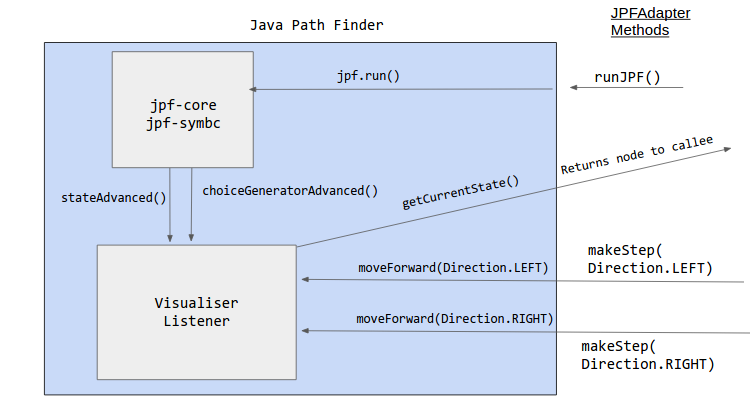
\includegraphics[scale=0.6]{inside_jpf.png}
\caption{Inside JPF - our \texttt{VisualiserListener} class}
\end{figure}

The \texttt{VisualiserListener} is our primary point of contact with JPF while it is running. This makes it one of the most crucial parts of our application. As mentioned earlier, the listener follows an event-driven programming paradigm. JPF executes the user's Java program and for every event, calls the corresponding listener function. Some events for which the listener is notified include \texttt{stateAdvanced()}, \texttt{stateProcessed()}, \texttt{stateBacktracked()} and \texttt{searchFinished()}. We override the implementations of these methods in our listener to suit our application's needs. In particular, we focus on two methods where the majority of the functionality is implemented. \\

The method \texttt{stateAdvanced()} is called when the program state changes. This is tracked through JPF's internal \texttt{SystemState}. The internal state contains a lot of redundant information for VISiBLE's purposes. As a result, we create our own \texttt{State} which represents a decision point in the program; each state corresponds to a node in the execution tree. The new state is created via a call to \texttt{createNewState()} which stores the state \texttt{id}, a reference to the parent state, an optional error message (empty by default) and the path conditions to each of its children (initially unknown). \\

JPF resumes executing the program once we return from the \texttt{stateAdvanced()} method. This leads to our next listener event of interest being triggered - \texttt{choiceGeneratorAdvanced()}. As mentioned earlier, a choice generator can refer to multiple choice types such as branching points, thread choices or random number choices. For our application, we are only interested in the first of these; JPF generates the possible path choices (the \texttt{if} and \texttt{else} case) at a branching point using a \texttt{PCChoiceGenerator}. \\

A path condition, represented by a String, is a set of boolean constraints that must hold for the program to have reached that execution point. The symbolic execution of the program, as performed by the \texttt{jpf-symbc} module of JPF, produces these for us. In \texttt{choiceGeneratorAdvanced()} we compute and assign each state their \texttt{ifPC} and \texttt{elsePC} - the next condition that must be true for us to take the \texttt{if} and \texttt{else} branch respectively. These path conditions are eventually displayed on the program tree in the front-end. \\

Another role of the listener is to handle the backend parts of the interactive side of our application. We achieve this via the use of latches as binary semaphores. While waiting for input from the user, we block JPF from executing. This is handled by the \texttt{movedForwardLatch}, which is set to 1 at every call to \texttt{moveForward} and counts down to 0 once we move forward. The thread running JPF busy waits while we are not allowed to wait forward - as we anticipate this to be a short duration, we feel this is justified despite the usual concerns of busy waiting. Further to that, we do not know how JPF handles threads internally; thus, we simply use JPF's \texttt{ThreadInfo} class, invoking it's \texttt{setSleeping()} and \texttt{setRunning()} methods on the current thread.

\paragraph{Using Docker to solve concurrency issues}

While JPF is a great tool, it does have one major problem; it cannot run multiple instances in the same JVM without the risk of them interfering. Undoubtedly, we needed to span multiple JVMs and the only issue remaining was how that can be done. \\

We aimed to provide a solution to this problem that would require as little hacking as possible, simple communication being our primary goal. We wanted something clean and reliable, even though we accepted these requirements might incur minor performance penalties. This set of specifications is what steered us away from spanning multiple processes and using inter-process communication (IPC). \\

The solution we went for is putting a copy of our web server which can run JPF in Docker \cite{docker} containers and allocate a Docker container for every user of our application. With this design, every program is being analysed symbolically in a different Docker container and hence a different JVM, without any possibility of interfering. \\

The communication becomes a pleasure to handle now. The primary web server only has the job of directing the user requests to the corresponding Docker container. This task is straightforward since the version of the web server running in the Docker container contains the same endpoints as our principal one. \\

Implementation wise, this is reflected by a different implementation of the \texttt{SymbolicExecutor} interface, the \texttt{DockerizedSymbolicExecutor}, which forwards the requests that reach the primary web server to the corresponding Dockerized server.
This implementation is elegant as Spring doesn't require us to create any mapping in between users and containers, but handles it through Bean scopes.

\subsubsection{Dependency Injection with Spring Beans}

Spring Beans are Java objects that are initialized, assembled and managed by the Spring Inversion of Control Container. \\

This concept allows for Spring to wire components together in a way indicated by a configuration file. \\

Our application provides a compelling use-case for Dependency Injection via Spring Beans. We are creating two separate instances of web servers. We have a web server which will run inside a Docker container, as well as the main web server, which will make the connection between a certain client and the Docker container running its particular instance of JPF. \\

Since both \texttt{JPFAdapter} and \texttt{DockerizedSymbolicExecutor} implement the \texttt{SymbolicExecutor} interface, we can register both of them as Beans and tell Spring which one to inject for every version of our application: the dockerized version will get \texttt{JPFAdapter} injected, while for the main Spring server will inject \texttt{DockerizedSymbolicExecutor}. This way, dependency injection allows our code to have entirely different behaviour without any change, illustrating the Open-Closed principle --- open to extension, closed to modification.

\subsection{Front-end} 
The front-end interacts with the user in following steps.
\begin{enumerate}
\item Get the input jar file.
\item Display all the methods in the program and then require the user to select a method to be executed symbolically.
\item Display a steerable tree corresponding to the method's symbolic execution. 
\end{enumerate}
At each of these steps, it also interacts with the back-end.

\subsubsection{Angular2 Application}
The front-end of the application is programmed using Google's \textbf{Angular2 web framework}\cite{angular}. 

\paragraph{Why Angular2}
We considered the web frameworks \textbf{Angular2} and \textbf{React JS} for front-end development. They both use TypeScript\cite{typescript} which allows for an object-oriented style which we have the most experience in. While both were strong options offering good speed and performance, community support and the ability to develop for all platforms, we opted for Angular2 because we had more experience using it.
Three members of our group had prior knowledge of Angular2, while one had programmed using Angular1 before.  \\

\paragraph{Application Overview}

The Angular2 application is a collection of \textbf{Components} and \textbf{Services} bundled under a root module. Components encapsulate the logic and structure of entities while Services fetch data for the Components. Components interact with each other and services are "injected" in components. It is the Component interaction, together with the use of services, that forms the front-end. The Components and Services of the front-end are as follows. \\

\textbf{Components:} 
\begin{itemize}
\item \texttt{App Component}: The top level Component that contains the Upload, Select and Tree Components, and coordinates between them.
\item \texttt{Upload Component}: Handles file upload from the user's machine to the back-end. It does so using the \textbf{ngx-upload}\cite{uploader} Angular2 uploader. The symbolic methods received in response to the jar upload are passed onto the Select Component.
\item \texttt{Select Component}: Displays and enables the selection of symbolic methods. Also allows the user to specify the arguments of the method that should be treated as symbolic by \texttt{JPF}. It uses the Tree Service to construct an initial tree which is passed onto the Tree Component.
\item \texttt{Tree Component}: Displays the visual steerable symbolic execution tree. Responds to the selection of an expandable node by branching at the node and displays the path conditions at each arc.
\end{itemize}

\begin{sidewaysfigure}
\centering
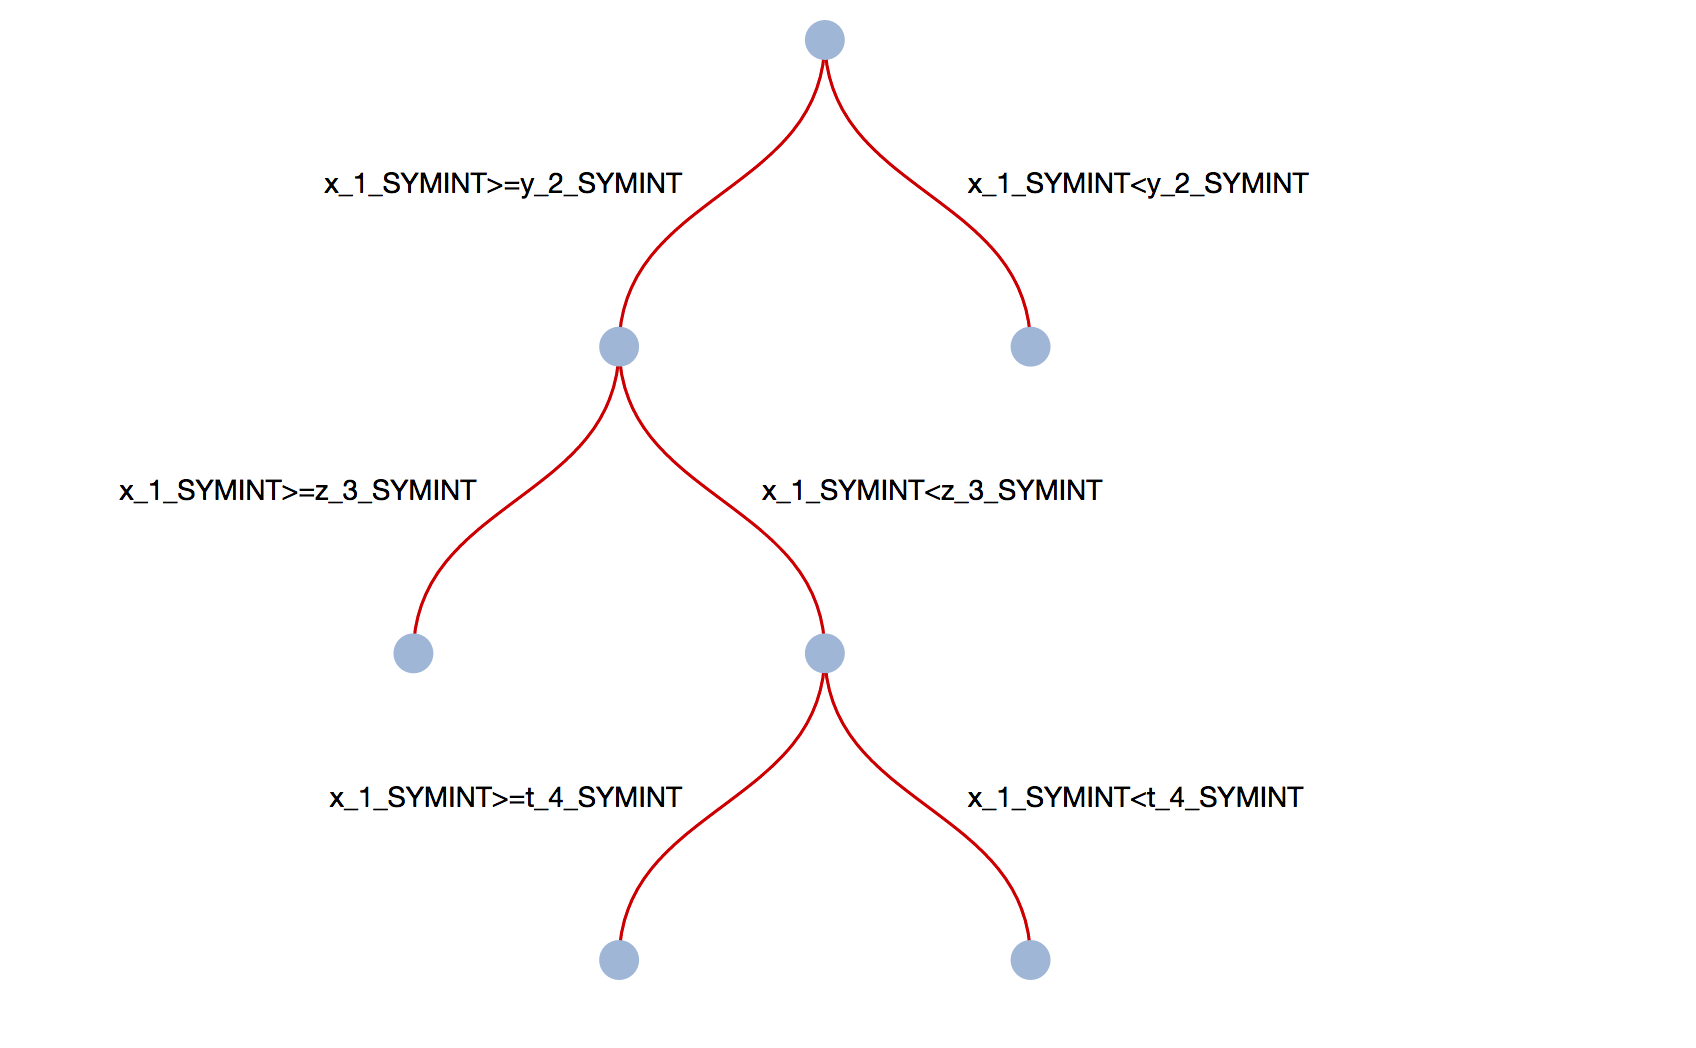
\includegraphics[scale=0.45]{d3-maxOf4.png}
\caption{Max Of Four Symbolic Execution}
\label{fig:visibled3}
\end{sidewaysfigure}

\textbf{Services}:
\begin{itemize}
\item \texttt{Tree Service}: The tree service interacts with the back-end and constructs a tree object which is then used by the \texttt{Tree Component} to display the tree. It further uses the \texttt{API Service} to make the Http requests to the back-end.

Used by the \texttt{Select Component} to generate the initial tree and the \texttt{App Component} to generate trees arising from steering left and right.

\item \texttt{API Service}: The API Service abstracts the details of making HTTP requests in Angular2, such as error handing, and object construction from response. It is intended that other services use the \texttt{API Service} to simplify their code, and have a sharper focus on their own specification. It is also used by the \texttt{Tree Service} for making HTTP requests to the back-end.

\end{itemize}

\textbf{Models:}

\begin{itemize}
\item \texttt{Node}: 
Recursive type represents a branching point. Stores path condition, and links to its children and parent.
\item \texttt{Tree}
A binary tree constructed from a root node.
\item \texttt{Method}
Represents a Java method. Stores its key information such its name, class name, signature and number of arguments.
\end{itemize}

Figure \ref{fig:frontend-arch} shows a high level component interaction sequence diagram.

\begin{figure}
\centering
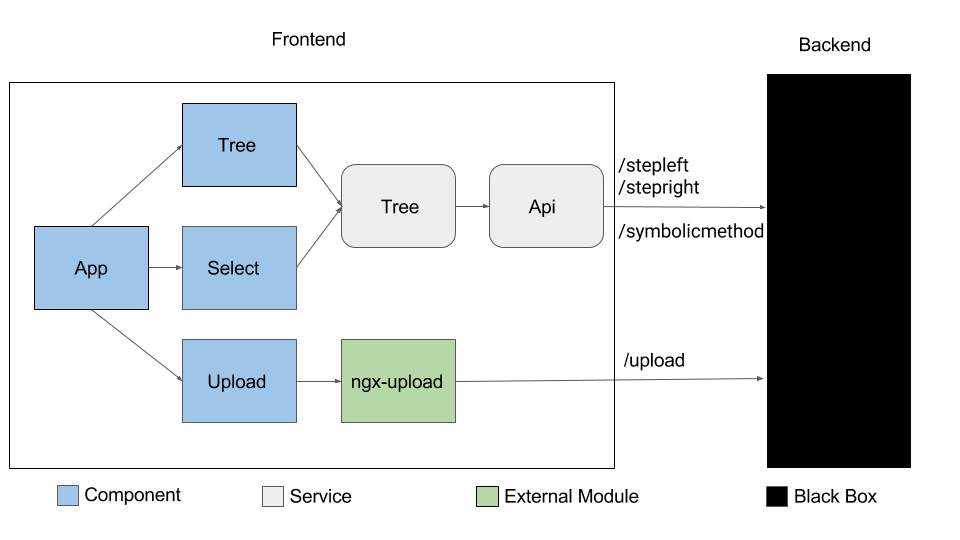
\includegraphics[scale=0.45]{frontend-architecture.png}
\caption{Hierarchy of Components and Services}
\label{fig:frontend-arch}
\end{figure}
    
\subsubsection{Drawing The Tree}
Apart from the initial file input and symbolic method selection, the front-end's sole job is to display and steer the execution tree. We would also like to have a scalable front-end such that it can handle drawing large trees. In this case, it would be desirable to avoid re-drawing the tree on each steer. It's also critical to manipulate the DOM, which is considered an expensive operation, in a certain degree of efficiency. These requirements had led us to choose D3 \cite{d3} library.

\paragraph{Why D3}

D3 \cite{d3} is a JavaScript library that is used to manipulate documents by binding itself to data. Once data is bound to a Document Object Model (DOM), its changes within the data will be reflected in the DOM. D3 is thus data driven and fits our needs of displaying a changing structure - the tree. It is also extremely fast, and since it draws using just the web standards HTML, CSS and Scalar Vector Graphics (SVG), it is compatible with all modern browsers. \\

With the flexibility of D3, comes a fair share of complexity too. There existed libraries, such as \texttt{PykChart.js}, which are based on D3 and easier to use, but are consequently slightly restrictive. We preferred flexibility and power over an easier learning curve. \\

We also considered the library \texttt{processing.js} which is based on the Processing visual language but with D3 having comparable capabilities, learning a new language was an overhead we did not need. \\

As a result, we decided on D3 in the end. Understanding and using D3 was a challenge but we eventually overcame.

\paragraph{Drawing The Tree With D3}
By passing in a node, by virtue of node being a recursive type, \texttt{D3} can deduce the nodes and links of the tree where the given node is the root node. This required us to define Node recursively.  The nodes and links obtained constitute the data values. These data values are then bound to HTML elements that represent the \texttt{svg} that draws circles for nodes, and lines for links.  Bound elements can be selected and their properties changed, and new DOM elements can be created for data values lacking a binding. \\

Starting from just the HTML \texttt{<svg></svg>}, constructing the tree can be broken down into three steps:
\begin{enumerate}
\item Defining the drawing area.
\item Drawing the nodes.
\item Drawing the arcs.
\end{enumerate}

\textbf{1. Defining the drawing area}. \\

This is done at the initialisation of the Tree Component. Height and width properties are added to svg tag and a group tag is nested inside it with a translate function. The role of the group and translate function is to create a padding for the tree from the defined \texttt{<svg>} bounds. The HTML at this stage, in pseudo Html, will resemble -
\begin{lstlisting}
<svg height: svg_height, width: svg_width>
  <g tranform: translate(dx, dy)>
</svg>
\end{lstlisting} 

\textbf{2. Drawing the nodes} \\

As explained above, passing in the root node of the initial tree to D3, returns the nodes corresponding the underlying tree. The HTML of these nodes is set to the \texttt{svg} that draws a circle and they are made a member of class \texttt{node} to enable grouping for CSS styling. \\

When step left or step right is called, the tree's left or right branch respectively is extended. This is done using the \texttt{Tree Service} and the extended tree is returned. D3 is able to detect the new nodes added to the tree, and again, the HTML of these nodes is set to the svg that draws a circle and they are  made a member of the class \texttt{node} for styling. \\

Also, for each node, an on-click event handler is defined. It checks whether the clicked node is expandable and if it is, expands the node by steering left/right. \\

In order to determine whether a node is expandable, we keep track of a current node. \\

The current node is the root node to begin with, and for every steer left/steer right operation, is the left/right child of the current node. With this notion of current node, an expandable node is the left or right child of the current node. \\

The parity of the node \texttt{id} then allows us to determine if the left or right child has been clicked for expansion. Accordingly, \texttt{stepleft} or \texttt{stepright} are called, and the current node is updated to the corresponding child. \\

\textbf{3. Drawing the arcs} \\
Again, passing in the root node of the tree, D3 returns the arcs for the tree. Similar to nodes, each arc is made a member of the \texttt{link} class for css styling, and it's HTML is set to the \texttt{svg} that draws a line. \\

The arcs also needed to be annotated with the path condition they represent.
This was straightforward as the arc object returned by D3 contained the source and destination nodes which in turn contained their own location. Adding an HTML text anchor between the two locations proved to be a simple and effective solution to achieve this.

\begin{lstlisting}

/* General d3 structure. */

// Get the d3 tree object
d3_tree = d3.layout.tree

// Get the nodes from the object.
nodes = d3_tree.nodes(rootNode)

// Bind data values to html 
node = svg.selectAll("node").data(nodes)

// Create html for data without a binding.
newNodes = node.enter().insert("node").on("click", expand())

// Add to html. 
newNodes.append("circle").attr("r", NODE_RADIUS).style("fill", NODE_COLOUR)
\end{lstlisting}

\subsubsection{General Design Decisions}
\noindent Decisions were made in the front-end to make the code modular, reusable and to speed up development. The following are the key ones that helped us with speedy and organised front-end development and that make the front-end extensible.

\paragraph{Mock Backend For Development}
\noindent Given the time taken for JPF to build, and the time it was taking us to understand JPF and come up with a working back-end, we decided it was best for front-end development to use a mock back-end. Once the integration end points were agreed, we constructed a simple mock back-end in \texttt{NodeJS} using the \texttt{Express} framework. Most of our development was done using this mock back-end. This way font-end development was fast, agnostic to the complexities of JPF and independent of the progress on the back-end.  

\paragraph{Separating Source Code From Transpiled Code}
\noindent One of the perks of using the Angular2 framework is to be able to program in TypeScript. The TypeScript is transpiled into JavaScript which is then run in the browser. By default, Angular2 compiles the JavaScript to the same directory as the TypeScript files. Since we would never need to modify these transpiled JavaScript files, we felt they cluttered the source code directories. So we directed the transpiled output to a new directory \texttt{dist/}

\paragraph{Shared Services And Models}

\noindent We tried to generalise our services and models so they may be used by multiple components. We generalised the data returned by a service by defining a model for it. For example, for the Tree Service, we created a Tree model and all service calls returned an instance of this model. We defined these services and models in a shared directory.

\section{Evaluation}

At the end of the project, VISiBLE presents a compelling set of features implemented in a clear, extensible way, providing an ideal code base for further extension -- the components of our code are highly cohesive but have low coupling.

\subsection{Deliverables}

We delivered a subset of the features we initially planned to implement. Working with legacy software which lacked documentation and a strong community had a lot to do with our failure to achieve the goals we set out for initially. It is the Agile development practices that allowed our project to remain a success, despite the unanticipated struggles we ran into along the way.

\subsubsection{Usability \& User feedback}

The software we developed offers an essential set of features, for anyone wanting to get an insight into the flow of their program. The ability to steer the execution and analysing the path condition at every step are core features. Despite a concurrency limitation of JPF which allows only a single instance to run in any particular JVM, our application successfully allows multiple users to symbolically execute their programs at the same time. \\

\noindent We have not yet spotted any bugs in the functionality mentioned above, in any of the runs we undertook. Our users who have tried the application have also reported it as being stable and bug-free although we did receive some complaints regarding the limited functionality. \\

\noindent The main issues highlighted by the members of Department of Computing who have tried our application was its limited usage, as we can only represent numeric values and booleans symbolically in its current version. \\

\noindent Another highly requested feature was giving the user the possibility to undo their last choice, as mis-clicks frequently occur. Since we have not yet implemented backtracking or the possibility to jump to any previously explored state, a mis-click requires our users to restart the execution of the program. \\

\noindent Despite those shortcomings, the stability of our software has been appreciated, as well as the capability to analyse the flow of the program in an intuitive way they have not experienced before. They regarded our tool as potentially very useful for debugging, were it extended with the requested features.

\subsubsection{Performance}

The features offered by our application require a lot of resources, as explained in [Design and implementation]. \\

\noindent The main bottleneck of our application is the implementation of JPF which does not allow several instances to run on the same JVM, as they can potentially interfere. This design flaw of JPF forced us to grow the number of JVMs we were using linearly with the number of users we have. It is therefore also required for us to scale our hardware together with our user base. \\

We chose the option of using web servers running in Docker containers instead of simple JVMs in order to avoid the struggles of interprocess communication, as detailed in [Design and Implementation]. This clean separation came at the cost of additional memory overhead. A container which just started running our server has an average memory consumption of around 310 \texttt{MiB RAM}, which increases once we start running JPF to around 380 \texttt{MiB RAM}. \\

We are currently running our application on Amazon's AWS EC2 \cite{aws}, on a machine featuring 4 \texttt{GB RAM}. As we cherish the reliability of our application, we felt the need to mitigate potential risks and chose a safe limit of only 6 Docker containers running at any given time. \\

While initialising a new container takes up to 10 seconds, this only happens when our server starts running. Afterwards, we are reusing already running containers to make the best use of our resources. We are thus able to serve our users quickly, the only delay being initialisation of JPF. It takes up to one second and is therefore not a concern for the user as our simple animation makes it evident that we are actively processing their request. We prevent our users from thinking we are providing suboptimal performance by making use of front-end routing. We thus ensure our users enjoy seamless transitions throughout the usage of our application.

\subsubsection{Code quality}

While developing the project we cared greatly about the quality of the code that powered our application. We enforced quality control using a thorough process of code reviews for pull requests, before merging into the \texttt{develop} branch. \\

\noindent During the group code reviews, we focused on the code being readable and extendable, avoiding depending on third party dependencies. We made extensive use of Spring's Inversion of Control container to manage dependency injection and object lifetime to help achieve our goal. This decision leads to us not having to manage dependencies manually, but let them in Spring's hands, leading to minimal coupling. \\

\noindent As an example of our project's modularity, there is no dependency on JPF either. As illustrated in the [Design and implementation] section, we are coding against an interface at all given times so that the implementation can be easily substituted. As a consequence, testing became much faster, as we mostly focused on the correctness of the messages sent, instead of the actual end-to-end behaviour. We will go into further detail about testing for both front-end and back-end in the next section. \\

\noindent For the front-end, we applied similar criteria, thanks to Angular's Dependency Injection mechanism. \\

\subsection{Testing}

Testing played a major part in our code development process, helping ensure correctness and serving as documentation alike. Continuous integration via Travis CI aimed to run the tests and evaluate whether our code was ready to be merged into our main branch. \\

\noindent While the unit testing was handled similarly in both front-end and back-end, there are bits which are specific to individual parts of our system. We will treat each one of these categories independently in the next subsections.

\subsubsection{Unit testing \& Integration testing}

\noindent For unit testing, as well as integration testing, we made use of well-established frameworks: Karma\cite{karma}, together with Jasmine\cite{jasmine} was our choice for the front-end, while JUnit \cite{junit} served our interests in the back-end. Alongside, due to our intense use of mock objects, checking the correctness of the sent messages was also a requirement. We used Mockito\cite{mockito}, which comes packed in Spring's testing module. Mocking the Angular2 components in front-end was done using testing utilities packed in Angular2. \\

\noindent We aimed to put together a test suite which runs quickly and achieves high code coverage. \\

\noindent We achieved fast testing by focusing on isolated components, replacing the dependencies of each class with mock objects. This separation minimised the computation each of our tests had to do, while fully evaluating the correctness of our code. \\

\noindent In such an environment, JPF's time to start was no longer relevant, as we only needed it checked in the tests which were checking the correctness of our listener. For all the other scenarios, creating a mock \texttt{SymbolicExecutor} was all that we required. \\

\noindent For the front-end, running JPF was not necessary. A mock back-end serving test data at the end points was sufficient to test the correctness of the front-end. \\ 

\noindent We monitored test coverage by using specialised tools: JaCoCo \cite{jacoco}and Karma coverage respectively. These instruments provided us not only with the percentage of code that our test covered, but gave us further insights. Generated reports allowed us to see which are the exact lines that are not covered by our tests and we were able to strengthen our test suite further in a way that leaves no critical behaviour untested.

\subsubsection{Backend testing}

For our backend, we needed a way of checking that the requests that reach our web server behave as expected. With such tests, our frontend can safely treat the backend as a black box, whose implementation does not matter, the same way coding against an interface works. \\

\noindent Thankfully, the creators of Spring anticipated the need for such testing and provided mechanisms to make it incredibly easy. Wiring up all the required dependencies is done via the \texttt{@MockBean} annotation, which creates Mockito mocks and injects them in the components which require them. Similarly, we can wrap beans with a Mockito spy, by using the \texttt{@SpyBean} annotation. \\

\noindent Spring provides a \texttt{TestRestTemplate} class to ease making HTTP requests, offering versatile methods for interacting with our API. \\

\noindent As far as this side of the testing is concerned, we checked that argument parsing works correctly, that the controllers forward the right messages to their corresponding dependencies, in all possible scenarios and that we are safely handling illegal inputs. \\

\noindent Not all of our tests make requests to mock objects, however. Our integration tests run through a "production-ready" backend, aiming to check that the version of \texttt{SymbolicExecutor} we are going to use is providing the right output. These tests do not run as part of our default test suite though as it would slow down our process too much. We chose to separate them in a different Gradle task, integration-testing, in order to keep our regular test suite fast. \\

We undertook stress testing, as part of evaluating how many users can use our application concurrently. We expected this number to be low, as described in the previous section, as the number of Docker containers running our web server needs to grow linearly with the number of users. \\

There is a certain degree of subjectivity in this evaluation, depending on how much risk one is willing to take, which is the reason we carried out this test manually, rather than using a script. We were aware that while not having sufficient memory, JPF has observable non-desired behaviour, as described in the last paragraph of the section. We wanted to avoid this issue at all cost, so we chose a safer approach. \\

Our memory is reasonably small for every new Docker container initialised: ~310 \texttt{MiB} for a server not running JPF and ~380 for one that is running JPF, values obtained by running the \texttt{docker stats} command. We illustrate the results in figures \ref{fig:onejpf} and \ref{fig:threejpfs}. \\


\begin{figure} [H]
\centering
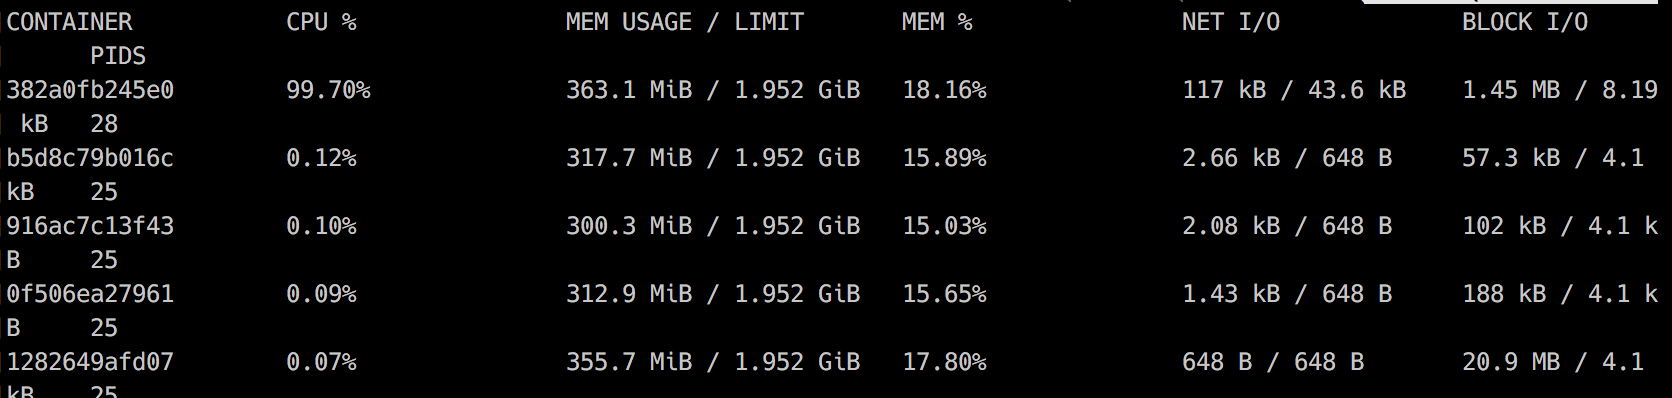
\includegraphics[scale=0.6]{onejpf.png}
\caption{Memory consumption when only the first container is running JPF}
\label{fig:onejpf}
\end{figure}

\begin{figure} [H]
\centering
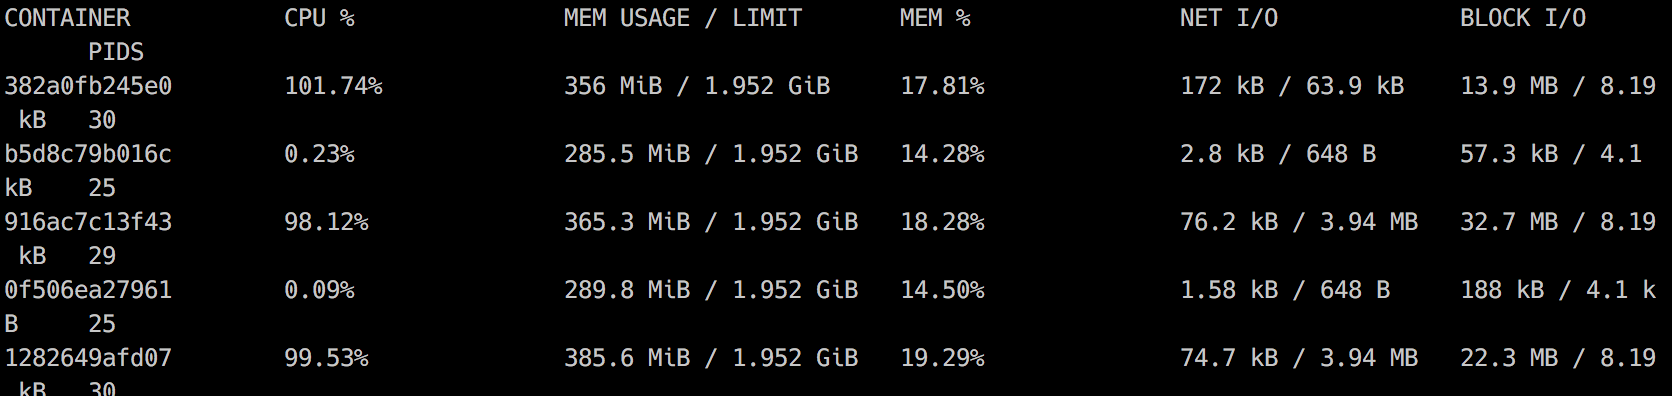
\includegraphics[scale=0.6]{threejpfs.png}
\caption{Memory consumption when three containers are running JPF}
\label{fig:threejpfs}
\end{figure}


We acknowledged that we carried out the tests for small, single class programs and the memory consumption will grow once JPF needs to keep track of a greater number of states. This observation led us to limit the number of Docker containers we create on our AWS EC2 4 \texttt{GB RAM} machine to 6. \\

We accidentally found out that JPF can skip a state when not having enough memory available, without producing any error. We discovered this bug while running the single-JPF version of our application on a \texttt{1 GB RAM} VM. We therefore strive to never put the system under memory stress, as we would not want our users to experience any non deterministic behaviour.

\subsubsection{Frontend testing}

While testing TypeScript code which simply processes data is a simple bussiness -- requiring nothing but the same old unit tests and mock objects, front-end poses its specific challenges. \\

\noindent Unlike any other parts of our system, we need to interact with a human user. In this aspect, a huge deal of non-determinism comes into play, as we need to handle multiple clicks, clicks in the wrong location, clicks while a resource is still loading and so on. While we were initially planning to use Selenium for testing these interactions, but we soon decided against it. The realisation that the user interface will change frequently in a short time frame and that would require rewriting a significant portion of the tests made us see writing the tests as being counter-productive. Instead, we chose to go for hand-testing, firstly using the application ourselves and later on offering it for other people to try. While testing this way does not provide for the same amount of accuracy as automated testing, we found the results satisfying. \\

\noindent The other aspect which makes the front-end of the application special is that it needs to interact with a back-end via HTTP requests. As we mentioned previously, we made extensive use of dependency injection in the front-end and back-end alike. As a consequence, we have the ability to swap in mock "service" classes, such that we now have to deal with requests to web servers in regular unit tests with mock objects.

\section{Conclusion and Extensions}

\subsection{Conclusion}

At the end of our project, after working together for more than two months, we managed to provide a useful extension to the JPF family, making symbolic execution more accessible to programmers, regardless of their experience level. \\

Our friendly, carefully crafted user interface can analyse all the paths of the program and provide useful test cases, which would direct the program execution to any particular line. Generating test cases and understanding the flow of a Java program has become easier due to VISiBLE. \\

We also benefited greatly from developing VISiBLE.
We are now comfortable with technologies we knew little about two months ago. The list includes, but is by no means limited to Java Spring, Docker, AngularJS. \\

We learnt a huge deal about teamwork and delivering software. The usage of Trello allowed us to be aware of progress in all parts of the project, while pair programming prevented bugs and helped make sure every member of the team has a good understanding of the way components interact. However, in developing our product, it is the customer involvement that we appreciated most -- our supervisor, acting as our client and mentor, proved to be invaluable for the development of our project, steering us back to the practices of Agile development every time we were falling in the trap of overly-engineering and under-delivering. We understood the need to know the customer and improve the product on a regular basis and certainly this is a lesson that is better to learn early. \\

It is dealing with legacy software that gave us the most headache throughout the development of the project. This aspect of the project is also the side of it from which we benefited most, being an experience we had not even once before. Our attempt to understand everything without constantly asking for help proved to be far from ideal, and it took us time to accept that understanding everything is not the target, but delivering a product is.

\subsection{Open source}

We are hoping that the project we developed can prove useful to the people in the JPF community and regular programming enthusiasts alike. To allow our product to become more useful, enhanced with valuable features, as presented in the next section, we will make our code open source and try bringing it into the eyes of the JPF community. \\

We believe this would be the best way for our project to grow, via feature requests, bug reports or involvement of additional developers. If the project were to generate enthusiasm, it would provide us with the extraordinary experience of managing a code-base over a longer period, with contributions from multiple individuals. \\

At the very least, the project would provide a useful insight into the workings of an otherwise poorly documented JPF. Our implementation might provide a starting point for many enthusiasts, looking to gain an understanding of JPF.

\subsection{Future development}

We feel that although our project does provide a minimal set of features, there is plenty of work yet to be done.

\subsubsection{Extending the range of supported types}

One of the most pressing issues of our application is that we can only handle numeric types and booleans symbolically. Supporting more types, was one of the main requests we have received from our users. \\

\noindent Supporting objects represents a real challenge. There are numerous attempts in the JPF community to solve this issue, for certain kinds of objects such as strings or sequences. Understanding how to make use of those would prove a great asset for our application, as we would be able to handle a much larger set of Java programs.

\subsubsection{Restore previously explored state}

Another feature which would be greatly appreciated by the first users of our software was the possibility of restoring any of the previously explored states. This addition would be a valuable guard against misclicks. Simply clicking on a state different than the desired one currently requires users to restart the symbolic execution of their program, a tedious, time-consuming procedure, which increases frustration and reduces the chances of them becoming returning users. \\

\noindent A feature which would partially solve the presented issue and is easier to implement is the possibility to backtrack to the previously explored state. While it obviously does not offer the tremendous level of flexibility of the ideal approach, it would relieve some of the pain experienced by our users.

\subsubsection{Smart visualisation}

Smart visualisation is one of the features which would make the project offer a better insight into analysed software. At the moment, there is no obvious connection in between the applications code and the symbolic tree displayed, which makes it hard for the user to make a connection to the stage of the program it is exploring now. \\

We would aim to give our users more context on the code they are symbolically executing through visual labelling. Questions such as "is this an if or a while" or "how many times have I iterated through this while loop" should be answered while symbolically executing code. \\

Implementing collapsible nodes or groups of nodes would also be useful, to allow users focus on the decisions in which they are truly interested. Another similar feature is a smarter positioning of the nodes, as in the current version of VISiBLE is handling trees with a large poorly and requires the user to scroll sideways.

\subsubsection{Non-deterministic choices}

The implementation of non-deterministic decision points would add a whole new dimension to JPF. One such additional type of decision point is thread scheduling. It would enable users to experience concurrency issues first hand, by making their program execute through any possible scheduling. The user should also have the option of choosing a thread scheduler and leave the execution of the program in its hands, controlling when the pre-emption shall take place or using a probabilistic model instead.

In the ideal version, the implementation design would allow the user to plug in their scheduling algorithm with relative ease. Such an option would prove useful for people who aim for extended low-level control over the execution of their program, seeking to understand the effects of different potential thread scheduling options.

\subsubsection{Stack/Heap visualisation}

Shifting the spotlight to education, we find stack and heap visualisation as being vital features. Together, they could provide those who are just starting their study of Computer Science with an immediate understanding of how memory management works, a problem known to baffle loads of beginners. This task would be challenging to implement due to the uncertainty induced by symbolic execution.

\bibliography{bib.bib}
\bibliographystyle{plain}

\end{document}